% Build: latexmk -pdf -interaction=nonstopmode -halt-on-error facet.tex
% Self-contained article. No external figures, fonts, or bibliography database.
\documentclass[11pt,a4paper]{article}
\usepackage[T1]{fontenc}
\usepackage[utf8]{inputenc}
\usepackage{lmodern,microtype}
\usepackage[margin=24mm,headheight=15pt]{geometry}
\usepackage{amsmath,amssymb,amsthm,mathtools}
\usepackage{stmaryrd}
\usepackage{booktabs,tabularx,longtable,array}
\usepackage{xcolor,listings,enumitem,fancyhdr,titlesec,needspace}
\usepackage{tikz}
\usetikzlibrary{arrows.meta,positioning,fit,calc}
\usepackage[most]{tcolorbox}
\usepackage{xurl}
\usepackage[colorlinks=true,linkcolor=blue!40!black,citecolor=blue!40!black,urlcolor=blue!40!black]{hyperref}
\usepackage{bookmark}
\definecolor{ink}{HTML}{203848}
\definecolor{accent}{HTML}{316D75}
\definecolor{pale}{HTML}{F1F5F5}
\definecolor{rulegray}{HTML}{CAD6D8}
\definecolor{muted}{HTML}{53626B}
\titleformat{\section}{\Large\sffamily\bfseries\color{ink}}{\thesection}{.65em}{}
\titleformat{\subsection}{\large\sffamily\bfseries\color{ink}}{\thesubsection}{.6em}{}
\titleformat{\subsubsection}{\normalsize\sffamily\bfseries\color{ink}}{\thesubsubsection}{.6em}{}
\titlespacing*{\section}{0pt}{3ex plus .6ex}{1.3ex}
\titlespacing*{\subsection}{0pt}{2.2ex plus .5ex}{.8ex}
\setlength{\parindent}{0pt}
\setlength{\parskip}{.38em}
\setlength{\emergencystretch}{2.5em}
\clubpenalty=10000
\widowpenalty=10000
\setlist{nosep,leftmargin=1.5em}
\setcounter{tocdepth}{2}
\renewcommand{\arraystretch}{1.15}
\newcolumntype{Y}{>{\raggedright\arraybackslash}X}
\newcolumntype{P}[1]{>{\raggedright\arraybackslash}p{#1}}
\newcommand{\code}[1]{\nolinkurl{#1}}
\newcommand{\R}{\mathbb R}
\newcommand{\N}{\mathbb N}
\newcommand{\Z}{\mathbb Z}
\newcommand{\Q}{\mathbb Q}
\newcommand{\C}{\mathbb C}
\newcommand{\den}[1]{\llbracket #1\rrbracket}
\newcommand{\Facet}{\textsc{Facet}}
\newcommand{\Spec}{\operatorname{Spec}}
\newcommand{\CertCheck}{\operatorname{check}}
\newcommand{\coeff}{\operatorname{coeff}}
\newcommand{\ecoeff}{\operatorname{ecoeff}}
\newcommand{\supp}{\operatorname{supp}}
\newcommand{\vct}[1]{\boldsymbol{#1}}
\newcommand{\source}[2]{\href{#1}{#2}}
\newtheorem{proposition}{Proposition}[section]
\newtheorem{theorem}[proposition]{Theorem}
\newtheorem{lemma}[proposition]{Lemma}
\theoremstyle{definition}
\newtheorem{definition}[proposition]{Definition}
\newtheorem{example}[proposition]{Example}
\newtcolorbox{designbox}[1][]{colback=pale,colframe=rulegray,boxrule=.5pt,arc=1mm,
  left=8pt,right=8pt,top=6pt,bottom=6pt,breakable,#1}
\lstset{basicstyle=\small\ttfamily,columns=fullflexible,keepspaces=true,
 breaklines=true,showstringspaces=false,tabsize=2,
 frame=single,rulecolor=\color{rulegray},backgroundcolor=\color{pale},
 framesep=5pt,xleftmargin=5pt,xrightmargin=5pt,aboveskip=.75em,belowskip=.75em}
\pagestyle{fancy}
\fancyhf{}
\fancyhead[L]{\small\sffamily Facet: objects, views, and certified computation}
\fancyhead[R]{\small\sffamily Second-round proposal}
\fancyfoot[C]{\small\thepage}
\renewcommand{\headrulewidth}{.3pt}
\hypersetup{pdftitle={Facet: Mathematical Objects, Explicit Views, and Certified Computation},
 pdfauthor={OpenAI, prepared for Vladimir Reshetnikov},
 pdfsubject={Second-round design of a Lean-hosted proof language and verified computer algebra environment},
 bookmarksnumbered=true}
\begin{document}
\begin{titlepage}
{\sffamily\small\color{muted}PROOF-LANGUAGE DESIGN \quad / \quad SECOND ITERATION\par}
\vspace{19mm}
{\sffamily\bfseries\fontsize{38}{43}\selectfont\color{ink}Facet\par}
\vspace{5mm}
{\sffamily\bfseries\fontsize{25}{31}\selectfont\color{ink}
Mathematical Objects,\\Explicit Views, and\\Certified Computation\par}
\vspace{10mm}
{\Large A representation-centered language over Lean,\\with a formally checked computer-algebra core\par}
\vspace{12mm}
\begin{designbox}
A mathematician should be able to keep referring to the same object while changing
how it is represented: as a finite sum, a generating function, a recurrence, a
factored polynomial, or a locally defined analytic expression. Each change must
say exactly what it preserves. Computation should produce such representations
and their evidence, not silently replace the mathematical question.
\end{designbox}
\vfill
{\large Prepared for Vladimir Reshetnikov\par}
{\sffamily 5 September 2026, Pacific time\par}
\vspace{5mm}
{\small\color{muted}
This is a technical design article, not a delivered language implementation.
The repository review is static. Proposed syntax, interfaces, and metatheory are
identified as specifications; the mathematical derivations are given explicitly.
Companion exact-arithmetic checks are executable tests, not Lean formalizations.
Repository revisions and the limits of the evidence are recorded in the article
and the source manifest.}
\end{titlepage}

\begin{abstract}
The first brainstorming round converged on a Lean-hosted language of mathematical
steps, scoped obligations, fixed statements, and replayable evidence. Its two
synthesis reports identify the remaining difficulties particularly clearly:
representation views do not yet have a satisfactory composition discipline;
method contracts risk duplicating ordinary theorem types; definitions may create
more friction than proof syntax; and a certificate that a theorem is true is not
necessarily a certificate for the explanation printed beside it.

This article proposes \Facet, an object-and-view layer whose primary operation is
\emph{a certified change of representation for a specified observation}. The
logical host remains Lean. The distinguishing design decisions are a separation
of exact presentations, restricted observations, and one-way abstractions;
support-sensitive composition without implicit strengthening; a typed protocol
for exact, conditional, branch-complete, and finite-precision computational
results; and a two-lane CAS architecture separating verified algorithms from
untrusted certificate discovery. Normalization becomes query-directed rather
than a single global normal form.

The design is grounded in ProveIt's binomial inversion, autonomous derivative,
and Bell generating-function developments, and in committed Leant source. A
worked EGF interface shows how to avoid repeated factorial cancellation while
retaining arbitrary commutative rational algebras. Further examples cover guarded
rational simplification, root isolation and radical denesting, local
differentiation, finite reindexing, and synthesis of proof connections. Concrete
interfaces, failure cases, an implementation sequence, and responses to all
twenty-two next-round questions in the two syntheses make the proposal testable.
No reduction in authoring time, proof length, or maintenance cost is claimed as a
measured result.
\end{abstract}

\tableofcontents
\clearpage

\section{The proposal in one argument}\label{sec:thesis}
\subsection{What the first round has already settled}
Both synthesis reports recommend retaining Lean, expressing meaningful
intermediate claims, giving omitted work exact scopes, fixing mathematical
meaning before proof search, and retaining accepted evidence. They also require
comparison with ordinary Lean equipped with the same helper libraries and
synthesis services. These are the right starting constraints, not contributions
that need to be invented again~\cite{synthesis,blueprints}.

The second round should answer a different question: \emph{what mathematical
abstraction should the shared infrastructure implement?} An obligation ledger
records work, but does not by itself reduce the work. A convenient spelling of
\code{have} makes a document easier to scan, but does not by itself explain why
an expression can be differentiated, why a rational coefficient may be cancelled,
or why a finite computation establishes an identity of infinite series.

My answer is to make \emph{objects and certified representations} first-class.
A mathematical argument typically retains an object while moving between
presentations selected for different purposes. A polynomial is factored to locate
roots, expanded to compare coefficients, and evaluated to establish a sign. An
integer sequence is studied through a recurrence, a generating series, and a
finite transform. A function is considered globally for a symmetry argument and
locally for a derivative calculation. A useful language must preserve the object
and make the change of viewpoint cheap, without confusing these different
notions of preservation.

\begin{designbox}
\textbf{Central design decision.} A computation or proof method does not merely
return an expression or close a goal. It returns a representation of a fixed
object, or evidence for a precisely named observation of that object, together
with the hypotheses under which that result is valid.
\end{designbox}

\subsection{The three distinctions that carry the design}
An \emph{exact presentation} denotes the same semantic object. A polynomial's
sparse coefficient list and its expression tree can be exact presentations of
one polynomial. A \emph{restricted observation} preserves only specified
information: a Taylor jet preserves finitely many coefficients; a germ preserves
local behavior; an interval enclosure preserves a containment fact. An
\emph{abstraction} supplies a directed logical implication and may lose information.
Reducing an integer equation modulo a prime is generally an abstraction, not a
reversible change of representation.

These distinctions are not cosmetic. If they are collapsed into one implicit
``view'' operation, the system can turn agreement of a finite prefix into equality
of sequences, agreement at a point into agreement near that point, or an equality
modulo a prime into an integer equality. Each of those is a different theorem.

The proposed language therefore keeps a stable semantic reference for the object,
lets the author select a useful representation or observation, and asks the
proof-producing infrastructure to construct the required bridges. This realizes
the first round's mathematical-step language without requiring every step to be
a new bespoke tactic.

\subsection{Why this is a proof assistant--CAS hybrid}
The CAS portion operates on certified representations of exact mathematical
objects. It can normalize polynomials, compute coefficients, propose factors,
isolate algebraic roots, and calculate bounds. The proof-assistant portion handles
quantifiers, arbitrary parameters, abstract structures, induction, local analytic
hypotheses, and the assembly of those computations into larger arguments.

There is no special ``CAS truth'' admitted by the kernel. Algorithms either have
proved correctness theorems and checked executions, or produce certificates for
verified checkers. Their inputs and outputs use the same object, context, and
observation protocol as ordinary theorem application. This is stronger than
asking a commercial CAS for an answer and then hoping a general tactic can prove
it. It is also more realistic than requiring every discovery heuristic to be
verified before the environment can benefit from it.

\subsection{What is new relative to the reports}
The first round already contains theorem-backed views, contextual holes,
semantic edit classes, and the separation of proof synthesis from data synthesis.
\Facet\ adopts those ideas. Its proposed increment is to give them a more concrete
mathematical and implementation boundary:

\begin{enumerate}
\item Exact presentations and information-losing observations have different
  interfaces, with explicit composition and reflection rules.
\item Computational results carry a precise specification, including domain
  conditions, branch coverage, and precision. Their evidence is tied to actual
  execution, not only to the correctness theorem of an algorithm.
\item A definition package supplies an observation interface, so recurring
  representation choices are resolved once rather than repaired in every proof.
\item Search is allowed to choose an implementation of an approved observation,
  but not its mathematical meaning. Leant can synthesize the connections between
  fixed interfaces, as well as individual proof terms.
\end{enumerate}

These are design contributions to this campaign, not claims of historical priority.
The relevant precedents are discussed in Section~\ref{sec:prior}. The first
implementation should be a Lean library and a small document layer. A separate
surface language earns its place only if the controlled comparison supports it.

\section{Evidence from the repositories}\label{sec:evidence}
\subsection{Snapshots and scope of the review}
Both requested TeX reports were read closely, including their mutual corrections
and next-round questions, at Brainstorm revision
\code{494be9d5ab41a5ae219fc6f800e6aee3c93bce39}. This is important: the questions
added to the second synthesis are included, not an earlier version of that report.
The individual proposals are used through the two syntheses' detailed crosswalks;
this article does not claim an independent full rereading of all nine proposals.

The directly inspected ProveIt files are at public revision
\code{24ce8bd743eaab64a91ce90725ea00f498d319d2}. The syntheses also discuss a newer
local checkout, \code{7c4e3f10}; those observations are attributed to the syntheses
rather than silently reassigned to the public snapshot. The inspected Leant
revision is \code{3a40904be8a410d832d9ab6900b3d3e7b425eccb}. Some findings in the
syntheses concern additional uncommitted working-tree changes. In particular,
their discussion of a new behavioral \code{where} clause is not treated here as a
fresh execution or as a feature verified in the committed source.

The review is static. Neither repository was built for this article. Bibliographic
entries identify paths and immutable revisions. The companion manifest records
which files and portions were inspected. This distinction matters more than a
large count of files allegedly ``reviewed.''

\subsection{Binomial inversion: the kernel identity, not the public corollary}
ProveIt's \code{BinomialInversion.lean} deliberately works at two levels: arbitrary
additive commutative groups acted on by integers, and commutative rings with
integer coefficients cast into them. The proof of kernel orthogonality passes
through interval conversion, shifted indexing, a binomial product identity,
natural-subtraction arithmetic, and cast normalization. The final inversion
results then reuse a lower-triangular transform calculus~\cite{p-binomial}.

The conclusion is not that the final theorem needs a more English-like spelling.
It is that the kernel calculation would benefit from a stable finite-sum view.
Inside the summand, the bound on the index should already be available to the
arithmetic transport. The coefficient identity should be proved over integers
and then transported forward, rather than rebuilding the calculation in every
coefficient algebra. At the same time, replacing this development by a
field-only CAS computation would lose one of its strongest properties: its
original generality.

\subsection{Autonomous derivatives: locality is mathematical information}
\code{AutonomousODE.iteratedDeriv_eq_comp} is already a compact proof. In the
successor case it converts the induction identity on an open set into an eventual
equality near the current point, transports the derivative, applies the chain
rule, and uses the recurrence. The hypotheses on the auxiliary functions are
required only at values actually reached by the solution~\cite{p-ode}.

This is an excellent semantic test, not a good source of exaggerated compression
claims. A frontend can present the argument as ``differentiate the identity
locally,'' but it must retain the neighborhood information and the range-local
hypotheses. Its benefit would be that the author handles a local function view,
rather than repeatedly spelling out the representation of eventual equality.
The source's existing proof remains a control against overengineering.

\subsection{Bell generating functions: a definition-level opportunity}
The additional example examined here is \code{BellShiftEGF.lean}, together with
the EGF interface in \code{BellGeneratingFunctions.lean}. It is particularly
useful because the second synthesis identifies EGF-related files as promising
places to investigate representation work~\cite{blueprints,p-bell,p-egf}.

The development represents an exponential generating function by an ordinary
formal power series whose coefficient is
\[
 [X^n]\operatorname{egfA}(a)=\rho(1/n!)a_n,
 \qquad \rho:\Q\longrightarrow A.
\]
Its abstract results work over an arbitrary commutative \(\Q\)-algebra. To extract
Spivey's identity, the source specializes the generating-function identity to
\(\Q\), applies the ordinary coefficient function, moves a common \(1/n!\) factor
through a sum, proves that factor nonzero, cancels it, and reflects the resulting
rational equality back to naturals~\cite{p-bell}.

The natural observation for that argument is not \([X^n]F\), but
\(n![X^n]F\). Giving that observation a proved interface removes the need to
introduce and then cancel the factorial normalization at each use. This is a
change of the definition's public interface, not merely proof-text compression.
Section~\ref{sec:egf} develops it completely and explains why it does not require
making \(A\) a field or making \(\rho\) injective.

\subsection{Leant: preserve the strongest boundaries already present}
Leant's committed \code{Verification.hs} explicitly says that its private
\code{Verified} wrapper records acceptance by a supplied callback, not a behavioral
proof, solver certificate, or kernel proof. The quota-aware scheduler groups
spellings of a candidate, stops at accepted quotas, and does not copy acceptance
authority from a merely equal-looking occurrence. These are useful boundaries
for the new protocol~\cite{l-verification}.

The fragment translator retains structural connectives, supported constructor
information, and typed application structure, while some dependent expressions
remain opaque. Its comments and safety machinery distinguish qualified negative
outcomes from unsuccessful bounded search~\cite{l-fragment}. The language should
reuse that distinction without elevating a safety flag into a formal theorem
about translation completeness.

Direct inspection of the committed suggestion path also confirms a narrower
issue identified by both syntheses. A probe runs one tactic, extracts possible
\code{Try this} replacement text, and may classify the result by a reduction in
visible goal count. The direct path does not independently replay that exact
replacement before caching it. A separate completion receipt is therefore needed
for the actual source edit, and current-goal progress must remain distinct from
whole-proof completion~\cite{l-main}. This is an interface requirement for a sealed
language, not a claim of a kernel soundness defect in an exploratory REPL.

\subsection{How much does the corpus audit establish?}
The second synthesis reports 90,637 classified tactic-like entries in 1,004
FabiusFunction files, with 29,303 entries in families it calls reconstructible.
The first synthesis independently reproduced its full-subtree summary fields.
Both revised discussions distinguish these lexical classifications from measured
removable work~\cite{synthesis,blueprints}.

I use that audit to select examples, not to predict a percentage saving. A cast
can be the mathematical substance of a theorem; a one-line solver call can hide
many failed attempts; an assertion can hide a substantial proof. Likewise, no
textual occurrence of \code{sorry} does not establish a successful build or an
acceptable transitive axiom inventory. The experiment must measure actual
obligations and author interventions, with semantic categories calibrated by
inspection.

\section{An object-and-view model}\label{sec:objects}
\subsection{Semantic anchors}
A semantic anchor is a resolved Lean object together with the environment and
ordered context in which it is meaningful. At the specification level write
\[
 a=(\mathcal E,\Gamma,D,d),\qquad \mathcal E;\Gamma\vdash d:D.
\]
The word ``anchor'' describes a reference discipline, not a new mathematical type
constructor in Lean. The same anchor may have several certified presentations.
Names and pretty-printed strings are not identities. A stored anchor must bind
universe parameters, type-class arguments, local instances, and the relevant
declaration dependencies as well as the expression's syntax.

The important restriction is that an algorithm cannot change \(D\), \(d\), or the
meaning-bearing part of \(\Gamma\) just because a different problem is easier.
It may propose a new anchor as an explicit definition or statement edit. Within
a calculation it normally proposes a new representation of the existing anchor.

\subsection{Exact presentations}
For a fixed semantic type \(D\), a presentation package has a representation type
\(R\), a validity predicate \(\operatorname{Valid}:R\to\mathrm{Prop}\), and a
meaning function
\[
 \operatorname{meaning}:\{r:R\mid\operatorname{Valid}(r)\}\longrightarrow D.
\]
A presentation of \(d:D\) consists of a valid \(r\) and an equality
\(\operatorname{meaning}(r)=d\). The validity predicate can be trivial. When it
is not, it contains genuine representation invariants: sorted exponents in a
sparse polynomial, reduced denominators in rational data, or an isolating interval
containing exactly one root of a nonzero polynomial.

It is often convenient to use a relation \(V(d,r)\) instead of a meaning function.
The functional form is preferable for the exact-presentation core because it
makes the preserved object unambiguous. Relational views remain available for
objects whose representation is only specified up to an equivalence, but the
relation and its transport laws must then be explicit.

A representation is not necessarily unique. Expanded and factored expressions
may both denote the same polynomial. The language does not demand a unique
canonical spelling for every mathematical object. It requires a certificate for
the representation actually chosen.

\subsection{Observations and restricted information}
An observation is a typed operation on an object, or a proposition about it.
Examples are the \(n\)-th normalized coefficient, evaluation at a point,
root-count in an interval, an upper bound, or equality in a germ at a point.
For a simple value-valued observation \(q:D\to B\), a computation can return
\[
 b:B,\qquad p:q(d)=b,
\]
without constructing a new exact presentation of all of \(d\).

Finite information requires this interface. A jet \(J_N(F)\) of a formal series
contains coefficients of degrees less than \(N\). Its certificate says exactly
that those coefficients agree with \(F\). It is not a certificate that the
truncated polynomial equals \(F\). Similarly, an interval \([l,u]\) is a certified
observation of a real value \(x\) when \(l\leq x\leq u\), not a replacement for
\(x\) by its midpoint.

One can describe a family of observations \(\mathcal O\) by
\[
 d\equiv_{\mathcal O}e
 \quad\Longleftrightarrow\quad
 \forall q\in\mathcal O,\ q(d)=q(e).
\]
Transport through this relation is allowed only for registered operations proved
to respect it. The relation is not inferred from the syntactic appearance of
later uses. Adding a new observation can invalidate an old replacement receipt.
For dependent observations, use a dependent transport theorem, not an untyped
list of equal scalar outputs.

\subsection{Supports and hypotheses}
The support of a computational result records where, or under what assumptions,
it is valid. Its logical content is an ordinary Lean proposition. Common supports
include \(x\in U\), \(j\leq k\leq n\), \(d\neq0\), or a neighborhood equality.
There is no separate unchecked ``CAS assumption database.''

A conditional presentation can have the form
\[
 S\longrightarrow V(d,r).
\]
It becomes available unconditionally in a local context only after \(S\) has been
proved there. If \(S\) cannot be proved, the system may retain a conditional result,
request a case split, or report that the selected operation is inapplicable. It
may not append \(S\) to the theorem's assumptions invisibly.

The support is not necessarily a nuisance. A nonzero denominator may be routine;
a domination hypothesis for a limit interchange may be the key mathematical
argument. The interface records their roles, but the theorem supplying the
operation remains authoritative about what is required.

\subsection{No change to definitional equality}
\Facet\ does not make CAS simplification part of Lean's definitional equality.
Expressions related by polynomial normalization remain propositionally equal
unless they were already definitionally equal in Lean. The elaborator inserts
checked transports where needed.

This avoids making conversion depend on an expanding collection of algebra
packages, nondeterministic search, or normalization budgets. It also prevents
accidental global changes to instance resolution. The compiler may share and
cache presentations aggressively, but the mathematical boundary is still an
ordinary theorem about ordinary Lean expressions.

\begin{center}
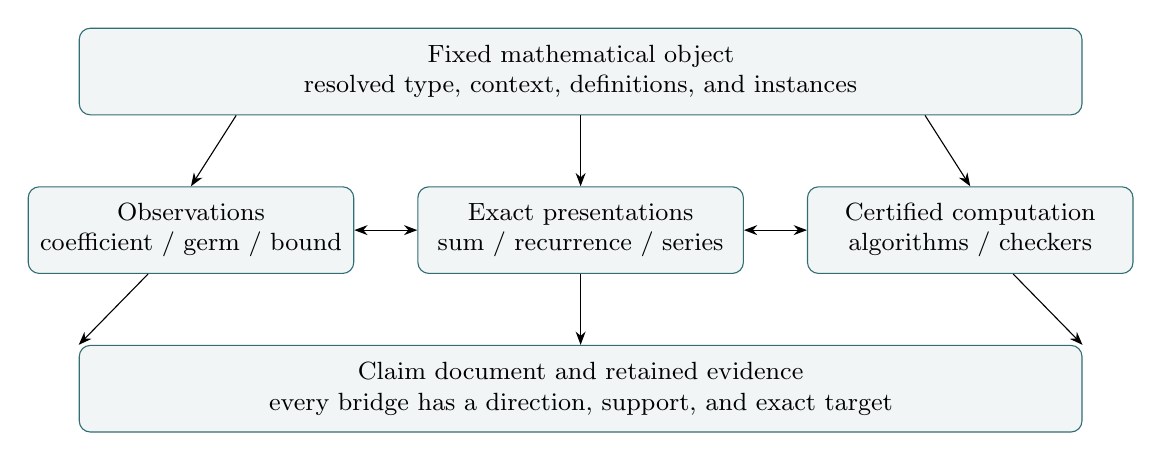
\begin{tikzpicture}[node distance=9mm and 8mm,>=Stealth,
 box/.style={draw=accent,fill=pale,rounded corners,align=center,font=\small,
 minimum height=11mm,text width=39mm}]
\node[box,text width=125mm] (a) {Fixed mathematical object\\resolved type, context, definitions, and instances};
\node[box,below=of a] (b) {Exact presentations\\sum / recurrence / series};
\node[box,left=of b] (c) {Observations\\coefficient / germ / bound};
\node[box,right=of b] (d) {Certified computation\\algorithms / checkers};
\node[box,text width=125mm,below=of b] (e) {Claim document and retained evidence\\every bridge has a direction, support, and exact target};
\draw[->] (a)--(b); \draw[->] (a.south west)++(20mm,0)--(c.north);
\draw[->] (a.south east)++(-20mm,0)--(d.north);
\draw[<->] (b)--(c); \draw[<->] (b)--(d);
\draw[->] (b)--(e); \draw[->] (c)--(e.north west);
\draw[->] (d)--(e.north east);
\end{tikzpicture}
\end{center}

\section{The language an author would write}\label{sec:surface}
\subsection{A small stored language, not unrestricted prose}
The initial frontend should reuse Lean expressions and binders, with a small set
of document commands around them. Mathematical notation is a rendering of typed
syntax. Free-form prose can explain an argument, but only formally marked claims
are assertions certified by the system. An assistant may propose source edits;
it does not interpret an unrestricted paragraph directly into trusted evidence.

The examples below are \emph{proposed syntax}. Names such as \code{EGF.coefficients}
and \code{rational.cancel} denote interfaces specified in this article, not
existing commands claimed to compile. Ordinary Lean proof blocks remain valid
leaves of the document and are checked under the same publication policy.

\Needspace{11.48\baselineskip}
\begin{lstlisting}
context (A : Type) [CommRing A] [Algebra Rat A]

object F : FormalSeries A := EGF A a

claim shifted : D F = EGF A (fun n => a (n + 1))
  by EGF.differentiate

observe c := ecoeff n F
  compute using EGF.coefficients

claim coefficient_value : c = a n
  from c.receipt
\end{lstlisting}

The \code{object} line introduces an ordinary definition with a stable semantic
anchor. The \code{observe} line fixes the expression \(\ecoeff_n(F)\) before
computation. Its result is not selected by searching for a conveniently provable
coefficient theorem. The receipt certifies that the returned value is the value
of that exact observation.

\subsection{Four verbs with different effects}
\code{Claim} introduces a proposition to prove. Any proof of that fixed proposition
is logically acceptable, subject to its dependency and method policies.
\code{Present} requests a new exact presentation of an existing object.
\code{Observe} computes a specified observation without claiming an exact
presentation of the whole object. \code{Select} chooses a new mathematical object
with a specification; this is a data-producing operation and may change all
later mathematics that refers to the selected object.

\Needspace{8.2\baselineskip}
\begin{lstlisting}
object roots : Set Real := {x | p.eval x = 0}

present roots as finite_algebraic_set
  compute using real_roots.complete

select r : Real
  satisfying p.eval r = 0 and 1 < r and r < 2
  using real_roots.unique_in_interval
\end{lstlisting}

The first computation owes both soundness and completeness of the returned root
set. The second owes a witness in the stated interval. If uniqueness is part of
the selection method, it also owes a uniqueness theorem. Merely producing one
root is insufficient for the first command. Merely producing any root is
insufficient for the second.

An existential proof used inside another proof is a different operation:
\code{obtain r with h from existence}. It performs scoped elimination in
\(\mathrm{Prop}\). It is not automatically an executable definition of a root.
Construction of a dependent pair in \(\mathrm{Type}\), propositional existence,
and a noncomputable choice operator retain their ordinary Lean distinctions.

\subsection{Calculations name the representation and the relation}
\Needspace{6.56\baselineskip}
\begin{lstlisting}
claim cancellation (x : Real) (hx : x != 1) :
    (x*x - 1) / (x - 1) = x + 1
  calculate over Real with support hx:
    (x*x - 1) / (x - 1)
      = ((x - 1) * (x + 1)) / (x - 1) by polynomial
      = x + 1 by rational.cancel
\end{lstlisting}

The first equality is a ring identity followed by congruence; the second requires
the nonzero denominator. The local support supplies that premise. A command
without \code{hx} can discover the conditional result, but cannot publish this
unconditional equality for an arbitrary \(x\).

The same expression can be explored without asserting the missing premise:
\Needspace{6.56\baselineskip}
\begin{lstlisting}
observe q := (x*x - 1) / (x - 1)
  compute using rational.cancel

-- Result, not an unconditional rewrite:
--   under x != 1: q = x + 1
--   unresolved support: x != 1
\end{lstlisting}
A publication can retain the conditional theorem as such. What it cannot do is
print \(q=x+1\) while keeping the premise only in a hidden warning.

\subsection{Domain changes are lexical and explicit}
A block such as \code{near x}, \code{over Rat}, or \code{coefficients below N}
changes the working observation or representation, not the original object.
The elaborated view shows the map used to enter the block and the theorem used
to leave it. There is no ambient convention that all functions are smooth or
that all denominators are nonzero.

\Needspace{5.74\baselineskip}
\begin{lstlisting}
claim derivative_step : HasDerivAt f v x
  near x:
    present f as g using local_identity
    derive g has_derivative v using chain_rule
  conclude by local_derivative_transport
\end{lstlisting}

Here \code{local_identity} must establish equality in a neighborhood, and the
last line names a theorem respecting that local relation. A pointwise equality
at \(x\) has the wrong type of information. The frontend can hide the proof that
an open set is a neighborhood, but cannot hide the absence of such a proof.

\subsection{Reasons: required, preferred, or unrestricted}
A named transformation in a \code{calculate} block is method-constrained by
default. If the author says ``reindex by this map,'' the method receipt must
contain that map, its coverage, and its summand correspondence. A different
proof of the equality is not a successful implementation of that explanation.

For an ordinary claim, \code{by search} means unrestricted reconstruction within
the stated policy. A \code{prefer} clause influences candidate order but does
not assert that the preferred method was used. The published rendering names
the actual accepted method. Changing a required reason is a visible plan edit,
not a silent tactic fallback.

This gives explanation a tractable meaning: the displayed method is the
instantiated proof constructor actually recorded. It does not pretend to prove
that the method was logically indispensable or that the proof reproduces a
human's internal reasoning process.

\subsection{References and incompleteness}
Authored claims receive stable identifiers. A printer may render a reference as
``the preceding identity'' only when that phrase resolves to the stored target.
Inserting a new identity does not silently retarget an accepted reference.
Copying a block creates fresh identities and checks the new scope.

Drafts may contain open claims, conditional computations, unsupported methods,
and proposed data choices. They are useful mathematical working documents.
Publication checks every formal assertion, including unused ones. A proof of
the final theorem cannot compensate for an unproved intermediate sentence.
Informal commentary is visibly distinguished from certified assertions rather
than being made to look equally checked.

\section{View composition, reflection, and coherence}\label{sec:views}
\subsection{Exact presentations compose without choosing a global normal form}
Suppose \(R_i,R_j,R_k\) present the same semantic type \(D\), with meaning maps
\(m_i,m_j,m_k\). A conversion \(f:R_i\to R_j\), on valid inputs, has a theorem
\[
 m_j(f(r))=m_i(r).
\]
A second conversion \(g:R_j\to R_k\) has
\(m_k(g(s))=m_j(s)\). Ordinary equality transitivity yields
\[
 m_k(g(f(r)))=m_i(r).
\]
This is the basic composition rule. The intermediate representation is concrete
and its invariants must be checked before the next conversion uses it.

\begin{proposition}[Anchor-relative coherence]\label{prop:coherence}
Let two accepted routes from an anchored object \(d:D\) produce presentations
\(r:R_i\) and \(s:R_j\), with proofs \(m_i(r)=d\) and \(m_j(s)=d\). Then every
observation \(q:D\to B\) has
\[
 q(m_i(r))=q(m_j(s)).
\]
\end{proposition}
\begin{proof}
The two meaning equalities give \(m_i(r)=m_j(s)\). Applying \(q\) to that equality
gives the conclusion. No equality between the representation types or their
inhabitants is required.
\end{proof}

This is a useful, limited answer to the syntheses' coherence question. Two
factorization algorithms may return factors in different orders. If both
presentations denote the same polynomial, an observation of the polynomial is
unaffected. An observation of the order of the factor list is not an observation
of the polynomial unless a separate convention has made that order part of the
specified object. The latter is a data choice, and must not be silently changed.

\subsection{Conditional routes accumulate dependent supports}
The real problem is often conditional conversion. Write a route as
\[
 r_0\xrightarrow[G_1]{f_1}r_1
 \xrightarrow[G_2]{f_2}r_2
 \xrightarrow[G_3]{f_3}r_3.
\]
Here \(G_2\) can mention \(r_1\), and \(G_3\) can mention both the value and
invariants produced at earlier stages. The correct record is an ordered
telescope, not a set of pretty-printed predicates:
\[
 h_1:G_1(r_0),\quad
 h_2:G_2(r_0,h_1,r_1),\quad
 h_3:G_3(r_0,h_1,r_1,h_2,r_2).
\]
The instantiated route is checked as one dependent program. If the supports are
independent propositions, a conjunction is an adequate presentation. The
implementation must not assume that special case universally.

Guard generation does not grant a guard. It creates a proof obligation in the
appropriate context. Failed alternatives are rolled back before another route
is tried, including assignments to shared metavariables. After a route is
accepted, the concrete intermediate representations, support proofs, and method
versions are retained.

\subsection{A three-view example: natural arithmetic through integers to rationals}
Let \(a,b,d\in\N\), assume \(b\leq a\), \(d>0\), and \(d\mid(a-b)\). Consider
\[
 u=(a\mathbin{\dot-}b)\mathbin{\mathrm{div}}d\in\N,
\]
where both operations are the natural operations. A route may first transport
\(a\mathbin{\dot-}b\) to its integer difference, next embed in \(\Q\), and finally
represent exact division by rational division. It owes, in order, the bound
needed for subtraction, the divisibility fact needed for exact division, and the
nonzero denominator needed for the rational manipulation.

A safe implementation can reason through a witness \(k\) with
\(a-b=dk\). It proves that the natural quotient is \(k\), and that the rational
quotient of the casts is also the cast of \(k\). The equality then follows through
that common witness. It does not identify floor division with field division.
For \(a=6,b=0,d=4\), the cast of the natural quotient is \(1\), while the rational
quotient is \(3/2\). For \(a=2,b=3\), the natural difference is \(0\), not \(-1\).

A direct natural-to-rational route and the route through integers may coexist.
If both have the same anchored input, exact target observation, and discharged
supports, Proposition~\ref{prop:coherence} gives observational agreement. The
recorded route still matters for explanation, performance, and maintenance.
Adding a cheaper route must not change a source-selected representation or
silently discard one route's necessary support.

\subsection{Preservation is not reflection}
A homomorphism \(h:A\to B\) preserves an equality: \(a=a'\) implies
\(h(a)=h(a')\). To conclude \(a=a'\) from the equality in \(B\), injectivity or an
appropriate reflection theorem is needed. A ring normalization in a quotient
ring cannot establish an arbitrary equality in the original ring.

The adapter interface consequently distinguishes
\[
 \operatorname{preserve}:P\to Q,
 \qquad
 \operatorname{reflect}:Q\to P.
\]
Either direction may exist without the other. A \(\Q\)-algebra map is useful for
forward transport of rational identities even when no injectivity hypothesis is
available. The natural-number embedding into \(\Q\), in contrast, supplies the
reflection used at the end of a natural-number coefficient argument.

This distinction must be part of method typing, not only documentation. The
compiler may search for a chain of directed bridges, but it may not reverse an
arrow because the displayed formulas look similar.

\subsection{Information-losing views need an observation budget}
For a formal series \(F\), let
\[
 J_N(F)=([X^0]F,\ldots,[X^{N-1}]F).
\]
Equality of \(J_N(F)\) and \(J_N(G)\) permits comparison of coefficients below
\(N\), not arbitrary coefficients. Multiplication preserves this precision:
\(J_N(FG)\) depends only on \(J_N(F)\) and \(J_N(G)\). Differentiation consumes
one coefficient of precision: \(J_{N-1}(F')\) is determined by \(J_N(F)\) when
\(N\geq1\).

Substitution has its own contract. The simple truncated substitution rule is
valid when the inner series has zero constant coefficient: terms of outer degree
at least \(N\) cannot contribute below degree \(N\). More general admissible
substitutions, for example involving nilpotent constant terms, require a different
precision theorem. Merely knowing that the host's substitution is defined does
not establish the simple zero-constant precision rule.

Thus a view records not just its result type but its \emph{available observations}.
A demand for coefficient \(N\) cannot be fulfilled from a jet of length \(N\).
The system requests more precision or another representation. It does not turn
finite evidence into an infinite identity.

\subsection{Germs are projections, not global function identities}
Passing from a function \(f:\R\to\R\) to its germ at \(x\) forgets behavior away
from \(x\). An eventual-equality certificate identifies two germs, not two global
functions. The derivative-transfer theorem is an observation theorem respecting
that germ relation. The route from a global function to a germ is therefore not
entered into the exact-presentation graph for global functions.

The distinction also prevents a subtle error with domain restrictions. A formula
valid only on \(U\) can give a germ formula at \(x\) when \(U\) is a neighborhood
of \(x\). A membership proof \(x\in U\), by itself, does not do so. The transition
needs a neighborhood theorem, which openness may supply.

\subsection{An abstraction ledger is not an adequacy proof}\label{sec:negative}
Both syntheses rightly emphasize that negative results need more care than
positive candidates. One refinement is essential: a list of abstracted nodes is
useful diagnostic metadata, but neither its emptiness nor a provider's claim of
complete search is a proof of end-to-end adequacy.

Suppose a provider searches an abstract proposition \(A\) for a target \(P\).
A checked proof of \(A\) transfers positively through a checked theorem
\(A\to P\). A checked proof of \(\neg A\) transfers negatively through a checked
theorem \(P\to A\). Those are different arrows. Each must account for the exact
context and foundational policy.

There is a further distinction between \emph{non-derivability in a proof calculus}
and a proof of a negation. Complete intuitionistic propositional proof search
can fail to derive an arbitrary instance of \(P\lor\neg P\), but that failure
cannot be imported as \(\neg(P\lor\neg P)\). Indeed intuitionistic reasoning
already proves
\[
 \neg\neg(P\lor\neg P):
 \quad h\mapsto h\bigl(\operatorname{Or.inr}
   (p\mapsto h(\operatorname{Or.inl}p))\bigr).
\]
A syntactic search-completeness certificate is therefore not automatically an
object-level refutation. Leant's fragment-qualified outcomes should remain
qualified metadata unless an actual proof at the original negated Lean goal is
constructed. This proposal strengthens the provider boundary without alleging
that Leant currently makes this particular invalid inference.

\section{Contracts and the typed intermediate representation}\label{sec:contracts}
\subsection{Logical contracts are ordinary theorems}
The second synthesis's proposal to use annotated theorem types is adopted, with
one adjustment to its durability story. Binder names are better than positional
flags, but they are not stable identities across library refactorings. A
project-owned adapter should expose stable semantic roles and map them to the
current theorem through a typechecked wrapper~\cite{blueprints,synthesis}.

For example, a finite reindexing adapter exposes \code{source}, \code{target},
\code{map}, \code{covers}, \code{injective}, and \code{summand}. A new upstream
lemma name or reordered binder changes the wrapper, not every proof document.
The wrapper itself is ordinary Lean and its proof is charged to the shared
library. The logical type is never duplicated in an unchecked contract language.

Roles control authoring and presentation. They do not decide logical relevance.
A bijection proof is not automatically routine because its type lives in
\(\mathrm{Prop}\); it may be the point of the argument. The method policy can
attempt it automatically, but records both the proposition and what was used.

\subsection{Three kinds of method implementation}
\textbf{Theorem adapters} instantiate one theorem or a small composite theorem.
Their unsupplied binders become obligations. \textbf{Certified computations}
reify a supported input, run an algorithm or checker, and return evidence for a
specified relation. \textbf{Structural plans} use recursors, case splits, and
reductions with scoped subdocuments. Their motives and coverage are explicit.

All three return typed evidence, but they should not be forced into the same
implementation API. An attribute on a theorem is enough for the first kind, not
for the entire mechanics of a normalizer or induction elaborator. Conversely,
introducing a new symbolic method object for every ordinary lemma would add
unnecessary maintenance.

\subsection{A common obligation record}
The authoritative worker owns the elaborated expressions. An obligation is
conceptually
\[
 O=(\mathit{id},\mathit{origin},\mathcal E,\Gamma,T,
       \mathit{roles},\mathit{policy},\mathit{dependencies}).
\]
Here \(\Gamma\) is an ordered dependent telescope, \(T\) is the fixed expected
type, and the origin includes the source revision, anchor identities, and worker
generation. There are separate controls for available local facts, library
constants, and allowed transitive axioms.

The provider receives a closed request over that telescope or opaque handles
owned by the worker. Pretty-printed formulas may accompany the request for
retrieval or model prompting, but do not replace its identity. Restricting the
local context must retain the dependencies required to type the remaining
variables. It is not equivalent to deleting unwanted printed hypothesis lines.

\subsection{IR nodes}
A small typed document IR needs the following node families. The table describes
interfaces, not a proposed change to Lean's kernel.

\Needspace{8\baselineskip}
\begin{longtable}{@{}P{.18\textwidth}P{.35\textwidth}P{.39\textwidth}@{}}
\toprule
Node & Meaning & Required retained information\\
\midrule\endhead
Definition & Introduce an anchored term. & Type, value, instances, exported observations.\\
Assertion & Prove a fixed proposition. & Context, exact target, evidence, source identity.\\
Presentation & Denote the same object in a new representation. & Representation invariant, meaning equality, support.\\
Observation & Compute a property or value of an anchor. & Query, precision/domain, output specification.\\
Selection & Construct a new specified object. & Exact witness, behavioral specification, choice policy.\\
Method & Apply a required theorem adapter or computation. & Instantiated contract, actual inputs and sub-obligations.\\
Case/induction & Introduce scoped subdocuments. & Cover or recursor, motive, local contexts, all branches.\\
Lean leaf & Admit an ordinary Lean proof body. & Verbatim source plus its checked boundary and dependencies.\\
\bottomrule
\end{longtable}

A document is not simply a DAG while elaboration metavariables remain unresolved.
There may be shared data and instance constraints across several nodes. Such a
cluster is elaborated transactionally; its closed interfaces are frozen before
independent provider work begins. Evidence dependencies are then acyclic after
recursors are treated as checked term constructors, not circular proof promises.

\subsection{What is checked, and what is merely reported}
A receipt can report a discovered candidate, an accepted local proof, a checked
computational specification, method conformance, or successful independent
replay. These statuses are not interchangeable. In particular, a successful
callback is not promoted into a universal specification theorem.

Final document acceptance requires a proof of the exact theorem, evidence for
every asserted intermediate claim, typechecked definitions and selections,
accepted computational specifications, and the declared dependency policy.
Method-constrained nodes additionally require their advertised constructor.
Human explanatory value and fidelity of informal commentary remain separate
questions. The renderer must never display a single undifferentiated green state
that conceals these distinctions.

\subsection{The modest assembly theorem}
After the interfaces are closed, each node is an ordinary Lean term constructor
applied to checked predecessors. Dependent substitution gives a term at the
fixed final target; the final kernel check is retained deliberately. This is the
same relative soundness argument accepted by both syntheses, and it does not
need another elaborate metatheory chapter~\cite{synthesis,blueprints}.

The interesting obligations lie in preserving that argument's premises: exact
input identity, coherent supports, no scoped witness escaping, correct
reification, checked computation, complete branch coverage, and faithful
source-to-claim mapping. Sections~\ref{sec:views} and~\ref{sec:cas} specify those
boundaries more closely. They are paper specifications here, not a formal proof
of an implemented compiler.

\section{A verified computer-algebra architecture}\label{sec:cas}
\subsection{Queries first, algorithms second}
A typed query fixes an input type \(I\), output family \(O(i)\), precondition
\(\operatorname{Pre}(i)\), and relation
\[
 \Spec(i,o):\mathrm{Prop}.
\]
Examples include polynomial equality, a factorization with product equal to the
input, the complete set of real roots, a particular coefficient, or an enclosure.
The user-visible command chooses the specification. Providers choose how to
produce a value satisfying it.

``Simplify'' is too vague as the fundamental query. A factorization query can
specify equality of the product, but irreducibility is an additional property.
A normal-form query can specify a canonical ordering, but an equality query need
not require canonical output. A root query can request all roots or one selected
root. Different specifications require different certificates even if their
outputs look superficially similar.

\subsection{Lane A: verified algorithms and checked executions}
Suppose a pure algorithm has been defined and verified:
\[
 \operatorname{alg}:I\to O,
 \qquad
 \operatorname{alg\_correct}:\forall i,\ \operatorname{Pre}(i)
       \to\Spec(i,\operatorname{alg}(i)).
\]
This does not, by itself, certify an arbitrary value \(o\) returned by a native
executable called \code{alg}. One also needs a checked connection between that
execution and the logical function: for example
\[
 e:\operatorname{alg}(i)=o,
\]
or a verified evaluator, refinement theorem plus justified evaluation, or a
computation trace whose verified checker establishes the same relation.

This execution boundary is easy to overlook when saying ``based on formally
verified algorithms.'' Proving the source algorithm correct is one obligation;
showing that the value actually used is its result is another. \Facet's strict
profile requires both. Small calculations can use kernel reduction. Larger
calculations can use compact certificates or a verified trace checker. A more
permissive native-computation profile can exist, but its additional trust is
explicit rather than being advertised as the strict profile.

Lean's current validation documentation makes this distinction operationally
relevant: native computation can introduce computation-specific axioms, and
since Lean 4.29 the historical single \code{Lean.trustCompiler} name is no longer
a sufficient audit target. The policy must inspect the actual transitive axiom
inventory, not blacklist one remembered constant~\cite{lean-validation}.

\subsection{Lane B: untrusted discovery with a verified checker}
For difficult discovery tasks, define a certificate type \(C(i,o)\), a total
checker, and a soundness theorem:
\begin{align*}
 \CertCheck &: \prod_i\prod_o C(i,o)\to\mathrm{Bool},\\
 \operatorname{check\_sound} &: \forall i,o,c,\quad
 \CertCheck(i,o,c)=\mathrm{true}\to\Spec(i,o).
\end{align*}
An external CAS, Leant, a language model, or a specialized search program may
propose \((o,c)\). Its authority ends there. The exact output is accepted only
through a checked computation of the checker and its soundness theorem.
Malformed, oversized, or unsupported data is rejected before expensive checking.

The checker need not be complete: rejecting a valid but unsupported certificate
is an operational limitation, not a mathematical refutation. Its own cost must
also be bounded by input and certificate limits. Certificate checking can be
expensive, especially for expanded polynomials, and should not be called cheap
without measurement.

Both lanes can implement one query. A verified factorization algorithm and an
untrusted factor generator can return the same factorization specification.
The author sees the same mathematical result but can inspect different execution
and provenance receipts. This permits incremental development without confusing
a verified checker with a fully verified discovery engine.

\subsection{Reification is part of the mathematical boundary}
An algebra backend usually does not compute on arbitrary Lean expressions. It
computes on a reflected syntax of polynomials, rationals, indices, or series
operations. The reifier must supply the connection to the original expression:
\[
 \operatorname{denote}(e,\nu)=t,
\]
where \(e\) is reflected syntax, \(\nu\) is the exact typed interpretation of its
variables, and \(t\) is the anchored Lean term. The environment records the actual
coefficient ring and its operations, not just the printed name ``ring.''

For example, treating an uninterpreted real expression as an atom is safe for a
positive ring identity when its exact interpretation is retained. Treating
noncommuting matrices as commuting atoms is not. Erasing natural subtraction
into ring subtraction is not. Approximating an algebraic number by a floating
point constant is not an exact reification.

After computation, the result is decoded through a checked interpretation theorem
and assembled into the original target. A certificate for the wrong reified
expression is useless even when its internal arithmetic is impeccable.

\subsection{Exact, conditional, covered, and approximate results}
The mathematical result family is richer than success/failure:
\Needspace{6.56\baselineskip}
\begin{lstlisting}
Exact(output, proof_of_specification)
Conditional(guard_telescope, output, proof_under_guards)
Covered(branches, proof_of_coverage, branch_specifications)
Enclosure(bounds, error_or_containment_proof)
Unsupported(feature, source_node)
Exhausted(resource_observations)
\end{lstlisting}
These are the checked-side concepts. An untrusted provider sends candidate
payloads, not authority-bearing \code{proof_of_specification} fields that the
consumer simply believes.

A conditional result proves \(G\to\Spec(i,o)\). A covered result contains
conditions \(G_1,\ldots,G_m\), a proof that the current assumptions imply their
disjunction, and a result under each condition. If branches overlap and the query
specifies a unique value, consistency follows from the specification's uniqueness
theorem; otherwise a deterministic selection policy must be part of the output.
A piecewise result must use only data available in its branch.

An enclosure establishes a relation such as \(l\leq x\leq u\), possibly with a
specified rational error. It is not an equality to a decimal approximation.
The display may round for readability, but the certificate stores exact bounds.
A request for a strict sign may be discharged by an enclosure not containing
zero; an enclosure containing zero is inconclusive, not a proof of zero.

\subsection{Branch coverage is substantive evidence}
Consider the equation \(ax=b\) over a field. The usual expression \(b/a\) solves
it when \(a\neq0\). A complete solution-set computation must also handle
\(a=0,b=0\), where every \(x\) is a solution, and \(a=0,b\neq0\), where none is.
The equality \(a=0\lor a\neq0\) and the corresponding split on \(b\) are part of
the proof of coverage. A ``generic case'' answer is valid only as a conditional
answer until those exceptional branches are accounted for.

This generalizes to discriminants, parameter-dependent root multiplicities,
vanishing leading coefficients, and singular matrices. The language should show
these as mathematical branches, not obscure CAS warnings. Which branch an
algorithm finds first is not a convention for interpreting the theorem.

\subsection{What belongs in the first verified algebra core}
Start with exact integers and rationals, sparse polynomial operations, polynomial
evaluation and differentiation, finite coefficient convolutions, and small
certificate checkers for algebraic identities. These support the EGF and
reindexing examples without a general symbolic integration engine.

The next layer can add polynomial division with remainder, Euclidean algorithms,
root-count certificates, and rational interval arithmetic. Symbolic integration,
multivariate real quantifier elimination, and general transcendental identities
are later providers with their own precise domains. The language protocol does
not promise a universal algorithm for them. It makes unsupported cases and
conditional results useful rather than misleading.

Existing Lean and Mathlib automation should be reused where its evidence fits.
The current Mathlib \code{Polyrith.lean} documentation, for example, says that the
external Sage-based \code{polyrith} path is no longer supported after the server
shutdown and points to \code{grobner} as an alternative for polynomial goals.
A roadmap must not depend on the old hosted service being available. The
certificate interface itself should be backend-independent~\cite{polyrith}.

\section{Worked algebra: cancellation, roots, and denesting}\label{sec:algebra}
\subsection{Polynomial certificates say exactly what they say}
A useful algebraic certificate for a consequence of equations
\(f_1=\cdots=f_m=0\) is an identity
\[
 p=\sum_{i=1}^{m}q_i f_i.
\]
A verified polynomial normalizer can check the identity. Evaluating it in a
commutative ring proves that \(p=0\) whenever the \(f_i\) vanish. The discovery
engine may use a Gr\"obner basis, but the checker need not repeat that discovery.

This certificate establishes ideal membership. It does not by itself provide a
complete decision procedure for every semantically valid consequence over every
ring. An implication valid over the reals may also use order, radicals, or
nonzero factors. A more general certificate
\[
 d^k p=\sum_i q_i f_i
\]
proves \(p=0\) only with suitable cancellation evidence for \(d^k\). In a field,
\(d\neq0\) suffices. In an arbitrary ring, a nonzero element can be a zero
divisor, so regularity or unit evidence is needed. The query must name the
ambient algebraic structure.

The factorization specification likewise has levels. Checking that
\(p=c\prod_i f_i^{e_i}\) certifies a factorization. Certifying that each \(f_i\)
is irreducible requires additional evidence in a specified coefficient domain.
The display must not upgrade a product identity into a complete irreducible
factorization merely because an external routine calls its result ``factor.''

\subsection{A rational-function identity is not a total-function identity}
In the fraction field \(\Q(X)\), the identity
\[
 \frac{X^2-1}{X-1}=X+1
\]
is unconditional because \(X-1\) is a nonzero polynomial. When interpreted as a
formula in a real variable with total real division, the corresponding equality
is conditional on \(x\neq1\). At \(x=1\), the left-hand side is \(0\), whereas
the right-hand side is \(2\).

The fraction-field computation is still useful. It produces a presentation of a
rational function, plus an evaluation theorem on points where the denominator
does not vanish. The language keeps these as two distinct steps. It does not
pretend that equality in a fraction field is equality of every totalized
pointwise evaluation.

For differentiation at a point \(x_0\neq1\), continuity of \(x\mapsto x-1\)
supplies a neighborhood on which the denominator stays nonzero. Only then may
the rational-function simplification be used as a local function identity and
differentiated. This is a three-way interaction among algebra, support, and
analysis that a useful hybrid should handle without hiding the argument.

\subsection{A radical identity with an explicit algebraic certificate}
Consider
\[
 \sqrt{3+2\sqrt2}=1+\sqrt2.
\]
Put \(u=\sqrt2\) and \(v=\sqrt{3+2u}\). The real-root specifications provide
\(u^2=2\), \(u\geq0\), \(v^2=3+2u\), and \(v\geq0\). The algebraic part is the
polynomial identity
\begin{equation}\label{eq:denestcert}
 (v-u-1)(v+u+1)
   =\bigl(v^2-3-2u\bigr)-\bigl(u^2-2\bigr).
\end{equation}
The right side is zero, and \(v+u+1>0\). Cancellation therefore gives
\(v-u-1=0\), which is the desired result.

This is a particularly transparent CAS certificate: a polynomial identity plus
a sign fact. It shows why algebraic equations alone do not identify the intended
root. Replacing \(v\) by its negative still satisfies the squared equation but
violates the nonnegative-root specification. The denominator in the cancellation
certificate is not an incidental formatting detail; it selects the correct
consequence of the polynomial equations.

\Needspace{8.2\baselineskip}
\begin{lstlisting}
claim denesting : sqrt (3 + 2 * sqrt 2) = 1 + sqrt 2
  let u := sqrt 2
  let v := sqrt (3 + 2*u)
  have hu : u*u = 2 and 0 <= u by real_sqrt
  have hv : v*v = 3 + 2*u and 0 <= v by real_sqrt
  have balance : (v-u-1)*(v+u+1) = 0
    by polynomial_certificate using hu hv
  conclude by cancellation using balance and positivity
\end{lstlisting}

A direct square-and-nonnegativity method would be equally reasonable. The system
should not use a root isolator for this example merely to demonstrate its most
complicated subsystem. The certificate vocabulary makes both proof routes
available and their actual costs comparable.

\subsection{The same identity through algebraic-root presentations}
For a more general denesting or algebraic-number calculation, use a polynomial
and an isolating interval. Here both sides are roots of
\[
 P(X)=X^4-6X^2+1
\]
in \((2,3)\). A Sturm sequence is
\begin{equation}\label{eq:sturm}
 P(X),\quad 4X^3-12X,\quad 3X^2-1,\quad \frac{32}{3}X,\quad 1.
\end{equation}
Each term after the first two is the negative remainder of its two predecessors.
At \(2\), the signs are \((-,+,+,+,+)\), with one variation. At \(3\), they are
all positive, with no variation. The endpoints are not roots. A root-count
theorem therefore gives exactly one root in \((2,3)\).

For \(u=\sqrt2\), the inequalities \(1<u<2\) place \(1+u\) in \((2,3)\), and
substitution using \(u^2=2\) proves \(P(1+u)=0\). For
\(v=\sqrt{3+2u}\), we have \(4<3+2u<9\), so \(2<v<3\); its square equation
gives \(P(v)=4u^2-8=0\). Uniqueness in the interval proves the identity.

An exact real-algebraic presentation can thus store a nonzero integer polynomial,
rational endpoints, a root-count certificate, and the unique-root meaning.
Polynomial irreducibility is not required merely to identify a unique root in
an interval. Zero polynomials, endpoint roots, repeated roots, and the distinction
between distinct-root counts and multiplicities need explicit treatment in the
checker. They are not safely handled by assuming a generic square-free case.

A full real-root-set result needs a global completeness certificate as well as
individual isolating intervals. For example, a verified root bound and counts
on a disjoint interval decomposition can show that every real root was included.
A list of individually valid roots establishes only soundness of the list, not
completeness. Multiplicity annotations add another specification layer.

\subsection{Parameter-dependent radicals need branch-local statements}
For real \(x\), \(\sqrt{x^2}=|x|\), not unconditionally \(x\). A branch-complete
presentation is \(x\) on \(x\geq0\) and \(-x\) on \(x<0\), together with coverage.
For complex roots, even this order-based split is unavailable; a principal-branch
convention and its branch-cut conditions belong to the semantic object.

Consequently, a denesting provider should first state whether it is returning
an identity in an algebraic extension, a real-valued branch identity on a domain,
or a principal complex identity. These are not interchangeable outputs of the
same untyped simplifier. The initial implementation should support exact real
algebraic constants before attempting general parameterized complex radicals.

\subsection{Certified approximations stay useful without becoming equalities}
Numerical search can help isolate a root, propose an interval, or find a likely
factor. Its output is then checked by exact arithmetic. For a transcendental
function, a bracket \([a,b]\) plus continuity and opposite endpoint signs proves
existence of a root; a positive lower derivative bound on the interval can prove
uniqueness and a residual-to-error estimate.

For instance, if \(f(r)=0\), \(r,x\in[a,b]\), and \(f'\geq m>0\) throughout
the interval, the mean value theorem gives
\[
 |x-r|\leq \frac{|f(x)|}{m}.
\]
A rigorous interval evaluation of \(f(x)\) then gives a certified enclosure for
\(r\). The numerical algorithm suggests \(x\); the theorem and exact bounds
supply the claim. The proof requires the interval and derivative hypotheses,
not just a small floating-point residual.

\section{A complete EGF interface and the Bell example}\label{sec:egf}
\subsection{The coefficient convention should be a named observation}
Let \(A\) be a commutative \(\Q\)-algebra and let \(\rho:\Q\to A\) be its
structure map. Define
\[
 u_n=\rho(1/n!),\qquad v_n=\rho(n!).
\]
Because \(n!\neq0\) in \(\Q\), the rational identity
\((1/n!)n!=1\) transports forward to
\begin{equation}\label{eq:factorialunits}
 u_nv_n=v_nu_n=1_A.
\end{equation}
No injectivity of \(\rho\) is needed for this equation. In particular, these
arguments do not need to exclude a trivial coefficient ring. They use an
explicit inverse identity, not cancellation from a claim that a mapped scalar
is nonzero.

For a sequence \(a:\N\to A\), set
\[
 E(a)=\sum_{n\geq0}u_na_nX^n,
 \qquad
 \ecoeff_n(F)=v_n[X^n]F.
\]
These are the semantic definition and observation that the EGF presentation
package should expose.

\begin{proposition}[EGF coordinates over arbitrary commutative rational algebras]
For all \(a\) and \(F\in A\llbracket X\rrbracket\),
\[
 \ecoeff_n(E(a))=a_n,\qquad
 E\bigl(n\mapsto\ecoeff_n(F)\bigr)=F.
\]
Thus the EGF coordinate map is a bijection between sequences and formal series.
\end{proposition}
\begin{proof}
The first identity is \(v_nu_na_n=a_n\), by
\eqref{eq:factorialunits}. For the second, the coefficient of \(X^n\) on the
left is \(u_nv_n[X^n]F=[X^n]F\). Formal-series extensionality gives equality.
\end{proof}

This is a representation theorem with a genuine inverse, not an assumption that
the coefficient map into \(A\) reflects equalities from \(\Q\). The proofs of
rational scalar identities take place in \(\Q\), and their images are used in
\(A\).

\subsection{Product and derivative rules}
Define binomial convolution by
\[
 (a\star b)_n=\sum_{k=0}^{n}\rho\!\left(\binom nk\right)a_kb_{n-k}.
\]
Then
\begin{equation}\label{eq:egfrules}
 E(a)E(b)=E(a\star b),\qquad
 \ecoeff_n(FG)=\sum_{k=0}^{n}\rho\!\left(\binom nk\right)
                    \ecoeff_k(F)\ecoeff_{n-k}(G).
\end{equation}
To check the scalar factor in the second equation, use the rational identity
\[
 n!\frac1{k!}\frac1{(n-k)!}=\binom nk
 \quad(0\leq k\leq n)
\]
and transport it through \(\rho\). The finite-sum binder supplies the index
bound; it does not need to be rediscovered at each multiplication node.

For the formal derivative \(D\), the coefficient formula
\([X^n]DF=(n+1)[X^{n+1}]F\) gives
\begin{equation}\label{eq:egfderiv}
 \ecoeff_n(DF)=\ecoeff_{n+1}(F),
 \qquad D E(a)=E(n\mapsto a_{n+1}).
\end{equation}
This follows from \(n!(n+1)=(n+1)!\), again in the scalar map. Repeated
application shifts by any \(m\), with no analytic convergence question.

The source already proves the corresponding EGF product and derivative laws.
The proposed change is to make normalized coefficients an explicit, reusable
observation interface and to let the coefficient compiler work directly in it,
not to present those identities as new mathematics~\cite{p-egf}.

\subsection{A representation-specific algebra, not an invisible instance switch}
The sequence type \(\N\to A\) also has its familiar pointwise operations. Under
EGF coordinates, however, series multiplication becomes \(\star\), not pointwise
multiplication. The language must not silently replace the ring instance on raw
sequences when a proof would become easier.

Use named operations or a distinct wrapper type, such as a structure whose data
field is a sequence and whose multiplication is explicitly binomial convolution.
The presentation package identifies that algebra. A statement written before
entering the package does not acquire a different multiplication afterward.
The resolved-statement view shows which operation is being used.

A possible package declaration is:
\Needspace{9.02\baselineskip}
\begin{lstlisting}
presentation EGFCoordinates (A) on FormalSeries A
  representation := EGFSequence A
  meaning a := egfA A a.coefficients
  observation normalized_coefficient n := factorial n * coeff n
  laws := coefficient_inverse, series_inverse
  operations :=
    add      : pointwise_add
    multiply : binomial_convolution
    derive   : shift
\end{lstlisting}

Every listed law is an ordinary theorem. The package declaration organizes those
laws; it does not make a multiplication convention true by declaration.

\subsection{A coefficient compiler rather than a collection of ad hoc tactics}
A first coefficient compiler can recognize constants, sums, scalar multiples,
products, formal derivatives, and \(\exp(aX)\). It recursively compiles the
requested normalized coefficient into finite algebra, accompanied by applications
of \eqref{eq:egfrules}--\eqref{eq:egfderiv} and the corresponding base rules.
Unsupported subexpressions remain typed atoms or explicit obligations.

For example,
\[
 \ecoeff_n\bigl(C(c)\exp(aX)E(b)\bigr)
   =c\sum_{k=0}^{n}\rho\!\left(\binom nk\right)b_k a^{n-k}.
\]
Here \(C(c)\) is the constant series. The author chooses the coefficient
observation; the compiler supplies routine scalar transport and finite
convolution. It is not asked to discover Spivey's identity by arbitrary theorem
search.

A compiled rule is a theorem schema for all \(n\), not a finite table of tested
coefficients. For numerical coefficient queries, a precision-indexed jet is often
more efficient. The same observation protocol distinguishes these two modes:
a symbolic universal theorem and a computation at one fixed index.

\subsection{Represent the Touchard calculation as polynomial algebra}
Write \(U=\exp(X)\) and let
\[
 T_m(Y)=\sum_{j=0}^{m}S(m,j)Y^j,
\]
where \(S(m,j)\) are Stirling numbers of the second kind. Their recurrence gives
\begin{equation}\label{eq:touchard}
 T_0(Y)=1,\qquad T_{m+1}(Y)=Y\bigl(T'_m(Y)+T_m(Y)\bigr).
\end{equation}
For \(1\leq j\leq m+1\), the coefficient on the right is
\(jS(m,j)+S(m,j-1)=S(m+1,j)\); the zero coefficient and the upper endpoint are
checked separately using the usual zero-extension convention. These endpoints
are part of the polynomial representation's support law.

The formal derivative obeys \(DU=U\). Hence
\[
 D(T_m(U))=U T'_m(U),
 \qquad D(T_m(U))+U T_m(U)=T_{m+1}(U).
\]
The long derivative-and-shift calculation in \code{derivative_touchardExp} can
therefore be approached through an ordinary polynomial representation followed
by a proved evaluation/derivative bridge~\cite{p-bell}.

This is an example of query-directed form selection. The finite exponential sum
is useful for extracting coefficients; the polynomial in \(U\) is useful for
proving the derivative recurrence. There is no reason to insist that one be the
canonical form for both jobs. The exact presentation receipts connect both to
the same formal series.

No injectivity of polynomial evaluation at \(U\) is needed here: the polynomial
identity is transported forward to a series identity. Inferring an arbitrary
polynomial identity backward from equal evaluations would require additional
evidence and is not part of this method.

\subsection{The shifted Bell identity}
Let
\[
 B(X)=\sum_{n\geq0}B_n\frac{X^n}{n!}
\]
in EGF notation, interpreted through \(\rho\) in \(A\). The Bell recurrence
establishes \(DB=UB\). Induction gives
\begin{equation}\label{eq:shiftedbell}
 D^m B=T_m(U)B.
\end{equation}
The base case is \(T_0=1\). If the identity holds at \(m\), then
\begin{align*}
 D^{m+1}B
 &=D(T_m(U))B+T_m(U)DB\\
 &=\bigl(UT'_m(U)+UT_m(U)\bigr)B
 =T_{m+1}(U)B.
\end{align*}
This is exactly the mathematical structure preserved by the source proof.
The proposed frontend should expose this induction and recurrence, not hide them
inside a command named after the final theorem.

\Needspace{8.2\baselineskip}
\begin{lstlisting}
claim shifted_bell (m : Nat) : D^[m] B = T m (exp X) * B
  induct m:
    zero:
      conclude using T_zero
    successor m using ih:
      differentiate ih formally
      use B_derivative and Touchard.polynomial_recurrence
      conclude by commutative_algebra
\end{lstlisting}

The notation \code{D^[m]} here means iteration of the formal derivative, not
pointwise exponentiation. This interpretation is fixed in the expression layer.
It has no connection to analytically differentiating a convergent power series
unless a separate analytic bridge is invoked.

\subsection{Spivey's identity without the recurring factorial detour}
Apply \(\ecoeff_n\) to \eqref{eq:shiftedbell}. The left side is \(B_{n+m}\) by
\eqref{eq:egfderiv}. On the right,
\[
 T_m(U)=\sum_{j=0}^{m}S(m,j)\exp(jX),
 \qquad \ecoeff_r(\exp(jX))=j^r.
\]
The coefficient compiler therefore obtains
\begin{equation}\label{eq:spivey}
 B_{n+m}=\sum_{j=0}^{m}\sum_{k=0}^{n}
   S(m,j)\binom nk B_k j^{n-k}.
\end{equation}
As an identity in \(A\), the integers and naturals are interpreted through their
canonical scalar maps. To conclude the stated natural-number identity, instantiate
\(A=\Q\), normalize casts, and use the injectivity of the natural embedding into
\(\Q\). This last reflection is a separate bridge. It is not a property assumed
for every \(\Q\)-algebra.

\Needspace{7.38\baselineskip}
\begin{lstlisting}
claim spivey (m n : Nat) :
    bell (m+n) = sum j in [0..m], sum k in [0..n],
      stirling2 m j * choose n k * bell k * j^(n-k)
  work in Rat by faithful_nat_embedding:
    observe normalized_coefficient n of shifted_bell m
    present T m (exp X) as its finite exponential sum
    conclude by EGF.coefficients
\end{lstlisting}

The omitted work has a bounded, compositional specification: evaluation of a
polynomial as a sum, a finite coefficient convolution, rational scalar identities,
and cast reflection. The theorem statement and the finite bounds stay visible.
The source's use of a commutative rational algebra has not been replaced by a
stronger global field hypothesis.

\subsection{What this saves, and what it does not}
The repeated factorial manipulation is moved into an ordinary library interface
whose laws are proved once. The polynomial presentation similarly centralizes
finite-support and evaluation plumbing. The induction and the choice to use a
generating function remain authored mathematics.

This is a plausible reduction in representation work, not a measured authoring
improvement. Ordinary Lean given the same \(\ecoeff\) and polynomial interfaces
may become just as concise. The experiment must measure that baseline. If it
does, the correct result is a better library plus an optional readable document
view, not a claim that new syntax caused the improvement.

\subsection{Finite computation and analytic interpretation remain separate}
Checking \eqref{eq:spivey} for finitely many \((m,n)\) is a useful regression test.
It does not establish the universal identity. Computing a jet of \(B\) can answer
specific coefficient queries, but not \eqref{eq:shiftedbell} for all orders. And
a formal identity in \(A\llbracket X\rrbracket\) is not automatically an equality
of real functions at every \(x\).

A future analytic-series package needs convergence and evaluation theorems with
explicit domains. It may consume a formal identity as one input, but the
convergence hypotheses are additional obligations. The language must not make
the word ``series'' select whichever interpretation lets the proof close.

\section{Local analysis and finite sums in the same model}\label{sec:analysis}
\subsection{Preserving the autonomous-derivative theorem}
Let \(U\subseteq\R\) be open, and suppose \(W,\varphi:\R\to\R\) satisfy
\[
 W'(x)=\varphi(W(x))\qquad(x\in U)
\]
in the sense of an actual derivative-existence statement. Let \(G_n,H_n\) be
families such that, for \(x\in U\),
\[
 G_0(W(x))=W(x),\quad
 G'_n(W(x))=H_n(W(x)),\quad
 G_{n+1}(W(x))=H_n(W(x))\varphi(W(x)).
\]
Only derivative existence at the displayed range points is needed. The conclusion
is \(W^{(n)}(x)=G_n(W(x))\) for every \(n\) and \(x\in U\), matching the
relevant generality of the ProveIt theorem~\cite{p-ode}.

The induction invariant is the identity on all of \(U\), not just at the current
point. At \(x\in U\), openness turns that identity into equality of germs.
Differentiating the representative \(G_n\circ W\) gives
\[
 (G_n\circ W)'(x)=H_n(W(x))\varphi(W(x))=G_{n+1}(W(x)).
\]
Derivative transport through the germ equality gives the successor case.

\Needspace{10.66\baselineskip}
\begin{lstlisting}
claim all_orders : forall n x, x in U -> D^[n] W x = G n (W x)
  induct n retaining the identity on U:
    zero:
      conclude using G_zero
    successor n using ih:
      fix x in U
      near x using U_is_open:
        present D^[n] W as G n o W using ih
        differentiate using G_derivative_at_image and W_equation
        use G_successor
      conclude by local_derivative_transport
\end{lstlisting}

The author-visible decisions are induction, retaining the identity on \(U\), and
using a local composition. The generated work is neighborhood construction,
function composition bookkeeping, and exact theorem application. The system does
not introduce global smoothness of \(G_n\), nor replace an arbitrary \(W\) by a
canonical solution it happens to know how to differentiate.

\subsection{A failed local view should name the missing fact}
Replace the invariant on \(U\) by equality at one point. The local presentation
fails with a diagnostic of the form:
\Needspace{4.92\baselineskip}
\begin{lstlisting}
Cannot enter the requested germ presentation at x.
Available: f x = g x.
Required: f and g agree on a neighborhood of x.
The derivative method has not been attempted.
\end{lstlisting}

This is much more useful than a failed general search for the final derivative.
For \(f(t)=0\), \(g(t)=t\), and \(x=0\), the available point equality is true
while the derivative conclusion is false. The diagnostic explains the exact
semantic gap. A proposed repair that adds a neighborhood hypothesis is a statement
change unless it can be proved from the original assumptions.

\subsection{Bounded sums provide scoped arithmetic facts}
For integers \(n,j\) represented as naturals with \(j\leq n\), put \(m=n-j\).
The bijection \(i\mapsto j+i\) between \(0\leq i\leq m\) and
\(j\leq k\leq n\) gives
\begin{align*}
 \sum_{k=j}^{n}(-1)^{n-k}\binom nk\binom kj
 &=\binom nj\sum_{i=0}^{m}(-1)^{m-i}\binom mi\\
 &=\binom nj\,[m=0]=[n=j].
\end{align*}
The complementary case \(n<j\) is an empty interval. The language should not
pretend it is covered by the same natural-subtraction normalization.

Inside the transformed summand, \(0\leq i\leq m\) is part of the local telescope.
It supplies the index facts needed by binomial identities and casts. Reindexing
owes a bijection or multiplicity-aware alternative, and equality of corresponding
summands. A half-open replacement \(0\leq i<m\) fails coverage at the upper
endpoint. This is a failure of the advertised method even if a broad solver can
prove the final theorem by an unrelated route~\cite{p-binomial}.

\subsection{A finite-sum CAS can check telescoping certificates}
A useful additional finite method accepts a proposed antidifference \(G\) and
checks, on the exact summation range,
\[
 f(k)=G(k+1)-G(k).
\]
It then derives
\[
 \sum_{k=a}^{b}f(k)=G(b+1)-G(a)
\]
for the selected finite interval convention. A discovery engine may guess \(G\)
or compute it symbolically; the checker verifies the difference identity and
endpoint conditions. If \(G\) is rational, every denominator used at the interior
and boundary points must be covered by the support.

This method demonstrates a genuine CAS--proof-assistant division of labor.
The expensive discovery of an antidifference can be untrusted, while its use in
an inductive or combinatorial proof remains a small verified operation. It grants
no right to telescope an infinite series without the additional limiting theorem.

\subsection{Substantial analytic moves remain substantial}
Dominated convergence, differentiation under an integral, and analytic continuation
should initially be theorem adapters with explicit hypotheses. The language can
organize an integrable dominating function and the relevant local uniformity
facts, but cannot classify their existence as routine by default.

For example, the pointwise limit of
\(f_n=n\mathbf1_{(0,1/n)}\) is zero on \([0,1]\), while each integral is one.
Pointwise convergence alone therefore cannot justify exchanging limit and
integral. A good hybrid can compute those integrals and verify the counterexample;
it cannot obtain the invalid interchange by a CAS rewrite rule. This is exactly
where expressive supports matter more than terse syntax.

\section{Integrating Leant without conflating its services}\label{sec:leant}
\subsection{Two productive roles}
Leant has two relevant jobs: proposing proof-state edits and synthesizing typed
terms. The new environment should not collapse them into a generic ``prove''
endpoint. A tactic edit changes an elaboration state; a synthesized term is
checked at a fixed expected type. Both can help, but they carry different replay
requirements~\cite{l-main,l-fragment}.

For \Facet, the first integration target is term assembly across fixed interfaces.
Suppose the local context contains a neighborhood membership proof, an identity
on that neighborhood, and a derivative certificate for a representative. The
adapter library exposes ordinary theorems connecting these to the desired
derivative claim. Leant can synthesize the composition without being asked to
invent the neighborhood or change the theorem's domain.

The second target is bounded route synthesis. Candidate terms assemble
presentation converters and observation transport theorems, with their support
proofs. The route endpoints and direction are fixed. A successful route is
rechecked as a term in the authoritative Lean worker. Failure remains failure
to find a route, not evidence that the mathematical claim is false.

\subsection{An exact request boundary}
The Lean-side adapter owns \code{Expr}s and context declarations. A request to an
external provider contains a stable request token, immutable origin, allowed
provider inventory, a structural search representation, opaque atom handles,
and resource limits. The worker keeps the authoritative association between
handles and expressions. Rendered formulas are auxiliary data.

\Needspace{13.12\baselineskip}
\begin{lstlisting}
Request
  origin         : environment + source_generation + obligation_id
  context        : ordered typed telescope, owned by Lean worker
  expected       : exact type handle
  effect         : evidence | representation | observation | selection
  inventory      : explicitly allowed theorem/adapter handles
  limits         : total time, memory, steps, candidate and payload caps
  abstraction    : diagnostic map plus any checked transfer contracts

Candidate
  request        : original request token
  construction   : typed assembly recipe or candidate source
  proposed_edit  : optional exact source replacement
  observations   : search and resource metadata, without proof authority
\end{lstlisting}

The final candidate is elaborated or reconstructed against the original expected
type. No implicit declaration is added to make an unknown identifier meaningful.
Universe and instance arguments that determine the target's meaning have already
been resolved or generalized explicitly. Candidates cannot reinterpret an opaque
atom by supplying a new pretty-printed string with the same spelling.

\subsection{Structural synthesis is useful even with opaque mathematics}
A synthesis engine need not understand real analysis to combine
\(H_1\to H_2\), \(H_2\to H_3\), and a term of \(H_1\). It can treat the
analytic propositions as opaque typed atoms. This is precisely where structural
synthesis complements a CAS. The CAS checks a polynomial or coefficient relation;
Leant finds a short typed route from that relation and the contextual premises
to the next claim.

Dependent arguments remain a boundary. A route that chooses an index map or a
new witness may affect the types of later obligations. The worker must either
instantiate those arguments first or validate the whole dependent candidate as
one transaction. A product-of-independent-holes encoding cannot be assumed for
all mathematical methods. Unsupported dependent structure should remain visible
rather than be erased to obtain a false completeness claim.

There is no reason to rewrite the Haskell engines before measuring this use.
A Lean-native adapter owns meaning; the existing engines remain replaceable
candidate generators. The comparison with \code{exact?} and ordinary theorem
application should distinguish single-lemma lookup from genuine compositions.
If nearly all accepted cases are the former, a dedicated adapter may not justify
its cost.

\subsection{Exact displayed-edit replay}
For tactic suggestions, the accepted transaction is the \emph{exact edit proposed
to the author}, not the tactic whose diagnostic message happened to contain it.
The protocol is:
\begin{enumerate}
\item Probe a candidate in a disposable worker cloned from an immutable origin.
\item Extract the exact replacement source, preserving scope and layout.
\item Replay that replacement from the same origin in a clean proof state.
\item Record its actual residual obligations or its completed proof term.
\item Accept the edit only if the live document still has the same origin.
\end{enumerate}

A response with fewer visible goals means progress or closure of a local goal,
not automatically completion of the entire theorem. The checked result records
remaining goals, unresolved metavariables, admissions, root-term status, and
publication policy separately. Missing status fields cannot be interpreted as
success. A late response after undo may be saved as a stale proposal, but cannot
mutate the current proof.

This addresses the exact boundary seen in the committed \code{suggestTactic}
path without discarding its useful behavior: looking past the first nonclosing
candidate, trying short composed continuations, caching by origin, and preserving
the user's script after backend failure~\cite{l-main}.

\subsection{Data synthesis needs a specified observation or behavior}
For a proof of a fixed proposition, different accepted terms are normally
interchangeable as evidence. For a selected datum, type inhabitation alone is not
a behavioral contract. Two projections both inhabit \(A\to A\to A\); a constant
failure function can inhabit the type of an option combinator. A candidate must
meet the property that downstream mathematics actually uses.

Finite tests are useful for exploration but certify only their finite
propositions. A universal behavior claim remains a separate proof obligation.
The syntheses' discussion of Leant's experimental behavioral work motivates this
separation, but is not a report that this article executed that work~\cite{synthesis,blueprints}.

Not every witness inside a proposition needs user interaction. A proof of an
existential proposition may construct a witness automatically while keeping the
public proposition fixed. The stronger stability rule applies when the document
names a particular witness as part of its mathematical argument or exports it as
observable data. The accepted witness and its specification are then retained;
substituting a different value is not merely replacing a proof term.

\subsection{Ranking should minimize burden, not only syntax}
For representation and route candidates, record a cost vector rather than a
single unexplained score: unresolved mathematical choices, new supports, number
of conversions, expected checking cost, certificate size, and adherence to the
requested explanation. Deterministic project policies can order this vector.
The system should not prefer a ten-character answer requiring a new field
hypothesis over a longer proof in the stated ring.

Proof-only holes can usually stop at the first accepted candidate within policy.
For data selections with genuinely different allowed values, present meaningful
alternatives or require a canonical specification. The published artifact needs
the selected object and its evidence. Rejected alternatives belong in an optional
exploration log, not the logical dependency closure of the theorem.

\section{Definitions, packages, and collaboration}\label{sec:definitions}
\subsection{A definition package is an interface, not an automatic theory generator}
The proposed definition package contains an ordinary Lean definition, explicit
operation conventions, exported observations, representation invariants, and
proved bridge theorems. It also names simplification orientations and the methods
permitted to construct alternative presentations. It does not generate arbitrary
mathematics from a natural-language definition.

The first package should be the EGF coordinate interface of
Section~\ref{sec:egf}. Its scope is small enough to implement and rich enough to
exercise nontrivial instances, finite supports, formal derivatives, and faithful
versus nonfaithful scalar transport. A second package can handle polynomials and
real-algebraic constants. A general controlled-language definition compiler
should wait for evidence that these interfaces cannot be expressed conveniently
with ordinary Lean declarations and templates.

\subsection{The API should expose useful observations, not every representation detail}
For an EGF, normalized coefficients, formal derivative, and binomial convolution
are natural observations and operations. For a bounded function, point evaluation
and its bound may be the useful interface, while the internal subtype projections
are not. For an algebraic root, evaluation of a polynomial and interval membership
are useful, whereas the order in which a solver found its isolating interval is
not.

Hiding representation details is safe only through proved interface theorems.
A user can explicitly open an implementation view when those details matter.
That creates new dependencies. For example, reasoning about the precise list of
factors means later reordering that list can no longer be treated as invisible.
The distinction is analogous to an abstract data type, but the interface laws are
mathematical theorems and are available to proof reconstruction.

\subsection{Instances and universe parameters stay explicit at the boundary}
The semantic seal includes the resolved instances used by the object and its
observations. A new ring instance or different coercion route can change the
meaning even when the printed formula remains unchanged. A proved proposition
used as a local instance, such as a property of an already fixed structure, is
different from selecting a different operation-bearing structure.

Unresolved universe constraints are also not left for a remote search engine
to settle opportunistically. A polymorphic declaration generalizes the intended
universe parameters. A monomorphic query fixes them. The worker may reconstruct
implicit proof arguments, but not change a value's type universe or algebraic
interpretation because one candidate elaborates more conveniently.

\subsection{Versioning has two independent layers}
A logical adapter version identifies the theorem and its typed role interface.
An operational policy version identifies search bounds, normalization orientation,
ranking, rendering, and permissible automatic supports. One can change while the
other remains unchanged.

A project-owned wrapper gives stable role names across upstream refactoring, but
its actual type is still checked. Reusing the same role identifier with a different
type does not make old evidence compatible. The old environment remains pinned;
a migration constructs new evidence and compares the resulting semantic anchors
and theorem statements.

\subsection{Conflicting packages should not become a global rewrite soup}
Imports make packages available; they do not automatically activate every
normalizer and coercion policy in them. A source block selects an active profile
lexically or by a qualified method name. Two conflicting normalization conventions
require an explicit selection. Combining rewrite sets indiscriminately can change
termination, output form, and explanatory behavior even when each rewrite is true.

Restrictions on permitted dependencies and axioms can be intersected when profiles
are composed, provided the remaining context is still well typed. Capabilities
may be combined only after the active interpretation and method priorities have
been resolved. ``Last import wins'' is not an acceptable semantic rule. The
resolved profile is part of the receipt, so a collaborator sees which policy was
used without reconstructing an accident of import order.

\subsection{Migration from existing Lean}
A lifting tool can recover named claims from \code{have} blocks, calculations,
and local definitions, attach retained evidence, and render them as a document.
It should preserve opaque Lean leaves when it cannot recognize a method safely.
It cannot generally recover an author's intended explanation from a proof term.
A recognized method annotation must itself be checked against the extracted
proof boundary, or remain a proposed annotation.

The initial round-trip guarantee should cover a documented subset: anchored
claims, explicit definitions, calculations, and the specified method nodes.
Arbitrary metaprogram source is preserved verbatim rather than normalized into
invented prose. This gives an adoption path that does not require rewriting the
entire ProveIt corpus before obtaining a useful view of it.

\section{Publication, replay, and the reader's evidence}\label{sec:replay}
\subsection{One artifact, several projections}
A published \Facet\ proof bundle is specified to contain the source document, an expanded Lean companion,
the anchored statement and definition manifest, accepted step evidence, computation
certificates, package versions, the dependency and axiom audit, and a bidirectional
source map. The human argument, obligation view, and exact evidence view are
projections of those records, not independently maintained documents.

A hash identifies content and supports cache lookup. It is not a proof. On a
cache hit, the expected type, context identity, semantic anchor, and certificate
schema are checked before evidence is reused. A proof from a sibling case must
not be imported because its printed goal matches the current one.

\subsection{Search-free replay still performs computation}
Replay does not rerun theorem retrieval, CAS discovery, synthesis ranking, or
model calls. It checks retained terms and certificates against the pinned
contracts and statements. Evaluating a verified certificate checker is still
computation; ``search-free'' does not mean zero checking cost.

Some large results may be best stored as compact certificates rather than
expanded proof terms. Others are cheap to retain as terms with shared dependencies.
The protocol permits both while recording which execution boundary is used.
Replaying an arbitrary saved tactic is a different mode because that tactic may
perform fresh search or depend on changed simplifier state.

The source remains the authoring representation. In the original pinned
environment, the accepted term or checked certificate is the evidence authority.
After an upgrade, the old evidence remains a historical artifact; it is not
silently treated as valid in a new environment. Migration produces a new receipt,
compares statement and definition meanings, and reports changes to objects or
plans. There is no promise that serialized Lean internals are portable across
all versions.

\subsection{A practical trust boundary}
Lean already separates elaboration from its small logical checker; \Facet\ uses
that architecture instead of inventing a new foundation~\cite{lean-elab}.
Untrusted producers run outside the acceptance worker. The strict publication
profile checks exact targets, all formal assertions, computation evidence, and
a transitive axiom allowlist. For externally supplied executable proof code,
process isolation protects the checking environment as well as logical state.

Current Lean documentation describes independent rechecking and a comparator
workflow that checks against a separately supplied statement. These are relevant
precedents, not features this article claims to have implemented or run.
A local prototype can start with ordinary Lean checking and an explicit status
report, while preserving an interface that can support the stronger deployment
boundary~\cite{lean-validation}.

\subsection{Visibility should track mathematical decisions}
The default reader view shows the theorem, the main claims, induction motives,
selected objects, representation changes, and substantial support assumptions.
Routine proofs of already visible bounds can be collapsed. The derivative example
should show why local equality is available; the denesting example should show
which root is selected; the EGF example should show that coefficients are
normalized and formal rather than analytic.

Clicking a step expands its exact instantiated contract, obligations, their
sources, and the accepted evidence. The system can report that a true intermediate
claim was not used. It cannot silently drop an unproved assertion to make a
publication succeed. A method-constrained rendering states what operation was
checked, not a stronger claim that no alternative proof exists.

\subsection{Semantic notices are not missing hypotheses}
A statement using natural subtraction or total real division is not automatically
wrong. The renderer should disclose its interpretation. A cancellation command,
on the other hand, may owe a nonzero premise. These are different statuses:
a semantic notice invites meaning review; a contract obligation requires evidence.

A dismissal of a notice can be scoped to a statement or to an explicit project
convention. Its key includes the relevant expression and convention version,
so a changed operation does not inherit an unrelated dismissal. New notices
should be sparse and evaluated for false alarms. A linter that warns about every
division teaches the author to stop reading rather than improving fidelity.

\section{Implementation sequence and performance}\label{sec:implementation}
\subsection{The smallest useful deliverable}
The first deliverable is not a standalone parser with dozens of mathematical
verbs. It is a Lean package that implements anchored queries, ordinary theorem
adapters, a source-linked receipt, and two representation packages: normalized
EGF coefficients and exact polynomial expressions. Ordinary Lean and a minimal
step frontend consume the same interface.

The end-to-end acceptance case is one coefficient proof: author a generating
identity, apply the normalized coefficient observation, reconstruct the finite
algebra, retain evidence, and replay with discovery disabled. Its negative
neighbor changes the requested coefficient beyond the available jet precision.
This is a small enough slice to reveal whether the object-and-observation model
is actually useful.

\Needspace{11\baselineskip}
\subsection{Modules and ownership}
\Needspace{8\baselineskip}
\begin{longtable}{@{}P{.23\textwidth}P{.40\textwidth}P{.29\textwidth}@{}}
\toprule
Module & Responsibility & Must not decide\\
\midrule\endhead
Core anchors & Resolved terms, contexts, identities, closed query boundaries. & Which theorem the author meant.\\
Document IR & Claims, source maps, scope, method and selection nodes. & That an unchecked assertion is harmless.\\
Presentation registry & Meaning maps, observations, support and transport laws. & That a one-way map is reversible.\\
Method adapters & Stable role interface to ordinary Lean theorems. & That every proposition-valued input is routine.\\
Algebra core & Reflected syntax, exact operations, verified checking. & That numeric resemblance is equality.\\
Provider scheduler & Budgets, candidate streams, cancellation, stale origins. & Proof or specification acceptance.\\
Leant bridge & Structural translation and origin-preserving candidate exchange. & A new interpretation for an opaque atom.\\
Evidence publisher & Exact-target validation, certificates, dependencies, replay. & Cross-version compatibility without rechecking.\\
Renderer/editor & Meaning disclosures, views, editable proposed patches. & Semantic identity from pretty-printing.\\
\bottomrule
\end{longtable}

\subsection{Batching and sharing without weakening scope}
Reifying the same coefficient expression for every tiny obligation would be
wasteful. Cache reflected subexpressions and interpretation proofs inside one
fixed environment and context. Use DAG sharing for polynomial and series
expressions, and retain common scalar identities as ordinary lemmas.

For a coefficient calculation, batch finite scalar identities over the same
ring and index telescope. Do not batch across incompatible branch assumptions.
If obligations share unresolved data choices, resolve or transactionally check
that cluster first. Scoped caches carry the origin, active instances, profile,
and precision. A certificate at precision \(N\) can answer smaller coefficient
queries through a proved restriction rule, never larger ones by wishful reuse.

Normalization should be demand driven. Expanding \((X+1)^{100000}\) is a poor
way to answer its degree or leading-coefficient query. The observation method
can prove those facts directly from a compact representation. A factorized
polynomial may remain factorized until a particular coefficient requires an
expansion. The proposed economy is semantic, not a claim that all expensive
algebra becomes cheap.

\subsection{Budgets describe the entire interaction}
Per-tactic heartbeats are not an end-to-end deadline. The request budget covers
candidate enumeration, reification, subprocess execution, communication,
certificate parsing, checking, and exact displayed-edit replay. Limits include
memory, output size, number of candidate attempts, and branch count as well as
elapsed time.

The scheduler returns partial \emph{information} without partial \emph{proof
acceptance}: a checked conditional result, an accepted intermediate presentation,
or a located unsupported subexpression can be useful even when the full query
exhausts its budget. Cancellation cannot turn a missing final receipt into a
successful proof. Worker generations prevent stale results from being committed
after undo or a changed definition.

\subsection{Implementation gates}
\textbf{Gate A: one exact path.} The normalized-coefficient proof works through
ordinary Lean and through the minimal document frontend, using the same library.
Every output observation has a checked specification. Replay performs no discovery.

\textbf{Gate B: semantic neighbors.} Add finite jets, guarded rational evaluation,
and the local derivative adapter. Reject precision overreach, a lost denominator
condition, and pointwise-only equality with diagnostics naming the missing fact.

\textbf{Gate C: a CAS certificate.} Check the denesting polynomial certificate
and a univariate root-count example. Mutated signs, omitted roots, invalid
interval endpoints, and missing branch coverage must fail at their exact boundary.

\textbf{Gate D: synthesis.} Connect Leant for closed structural assembly and
bounded view routes. Run exact-source replay and stale-origin tests before
advertising verified tactic edits. Compare the closure and latency profile with
existing Lean alternatives.

\textbf{Gate E: authoring evidence.} Run the frontend and definition-package
comparison, including repair after library changes. Expand the grammar only
when a failed task demonstrates a need that cannot be met by a shared library
interface or a better document rendering.

These gates are deliverables, not a calendar estimate. They deliberately leave
large symbolic integration and general natural-language interpretation out of
the first implementation.

\section{Evaluation that separates language from library}\label{sec:evaluation}
\subsection{Three baselines and a representation ablation}
Use three primary conditions: idiomatic existing Lean; refactored Lean with the
same adapters, observation packages, CAS checkers, and Leant access; and the new
frontend over that same machinery. The difference between the last two measures
the surface and interaction layer. The difference between the first two measures
shared mathematical and automation infrastructure.

Add a representation ablation: perform the EGF tasks both with the original
ordinary-coefficient interface and with normalized coefficients, keeping the
frontend fixed. This tests the definition-package thesis independently of the
syntax thesis. An improved ordinary Lean proof is a successful outcome, not a
result to hide because it weakens a language marketing claim.

\subsection{Tasks and controls}
Use the inspected binomial and derivative examples as development tasks, and
Bell-related coefficient and recurrence tasks as a richer representation test.
Hold out entire theorem families or modules before tuning adapters. Include at
least one already-short corollary as a control: the new frontend should be
allowed to preserve its short Lean form.

A reading study asks participants to identify the central argument, locate an
essential assumption, and predict the effect of a mutation. An authoring study
records time, edits, unsuccessful attempts, explicit mathematical choices, and
new helper lemmas. A maintenance study changes an endpoint, a coefficient
convention, an instance, a theorem name, and a package version separately.
Frontend order should be counterbalanced, and Lean and domain experience recorded.

\subsection{Leakage and infrastructure costs}
Remove the target theorem and its downstream consequences from the permitted
retrieval environment. A cached proof, alias, example, or provider wrapping the
target is still leakage. Split by theorem or module before harvesting subgoals,
not after near-identical goals have entered the training or tuning corpus.
Record the exact environment and dependency exclusions for every task.

Charge for all new mathematics, wrappers, checker proofs, parser work, and
maintenance. For \(n\) tasks, report
\[
 C(n)=L+\sum_{i=1}^{n}(A_i+R_i),
\]
where \(L\) is shared infrastructure cost, \(A_i\) is authoring effort, and
\(R_i\) is repair effort under the defined mutations. Do not amortize \(L\)
over hypothetical future users. Report the components and observed reuse.

\subsection{Measures and decision criteria}
Source length, generated term size, and bridge counts are useful descriptions,
not universal utility measures. Record median and tail interaction latency,
checking time, certificate size, support obligations needing author input,
reader accuracy, and repair effort. Publish failed tasks and false-positive
notices as well as successful demonstrations.

Exact statement preservation, scope safety, precision discipline, and the required
negative-case behavior are hard correctness gates. Usability thresholds should
be chosen after a pilot provides actual variance, not invented in this article.
If normalized coefficients help but new syntax does not, ship the coefficient
library. If the document view helps readers but slows authors, offer it as a
rendering. If the method registry costs more to maintain than its saved work,
reduce its scope rather than conceal the cost in generated files.

\section{Relation to existing work and limits}\label{sec:prior}
\subsection{Relevant precedents, without claiming a new foundation}
The immediate intellectual source is the nine-proposal campaign as evaluated by
its two syntheses. The claim-and-obligation layer, statement locks, method
conformance, and fair shared-library baseline are adopted explicitly, not
presented as new discoveries~\cite{synthesis,blueprints}.

CoqEAL is a relevant precedent for connecting mathematical representations with
more efficient computational ones through refinement. Its project separates
abstract algebraic material, computation-oriented data structures, and a
refinement framework. \Facet\ proposes a language-facing organization around
that general kind of representation discipline, not the invention of verified
representation changes~\cite{coqeal}.

Li, Passmore, and Paulson's work on univariate polynomial problems in Isabelle/HOL
separates external certificate discovery from formally checked real-algebraic
reasoning. The associated Sturm--Tarski formalization is a concrete precedent
for the root-count lane. These are Isabelle developments, not evidence that a
matching Lean implementation is already present. Their execution and code-
generation trust boundaries must be assessed in their own setting; citing them
does not supply a strict Lean execution receipt~\cite{univariate,sturm}.

The design's distinctive emphasis is the shared source-level protocol: an
algebraic certificate, a local analytic identity, and a normalized coefficient
computation all report what observation they establish of which fixed object,
on what support. It is an integration and interface proposal over an existing
logical foundation.

\subsection{What is established in this article}
The algebraic and EGF derivations are supplied as mathematical arguments. The
Sturm-chain arithmetic and small finite identities are independently exercised
by the companion exact-arithmetic program. The repository observations are
static source readings at recorded revisions. The design provides concrete
contracts and tests, not an implemented compiler or a Lean-verified metatheory.

In particular, no claims are made here that the proposed syntax compiles, that
the new CAS checkers have been formalized in Lean, or that authors become faster.
No ProveIt or Leant build or live backend acceptance suite was run. The companion
program is a regression aid and certificate illustration, not a replacement for
the verified checker that the implementation would need.

\subsection{The central risk and the useful fallback}
The main risk is not that Lean lacks a place to check the evidence. It is that
creating and maintaining observation interfaces costs more than the authoring
friction they remove, or that the interfaces hide the very distinctions readers
need. The scoped examples and controlled evaluation are designed to test that
risk directly.

The useful fallback is substantial: normalized coefficient interfaces, stable
adapters, exact suggestion replay, and better source-linked evidence can all
improve ordinary Lean without a new language becoming the primary input form.
The proposal is therefore not contingent on inventing a more English-looking
syntax. Its technical hypothesis is that mathematical objects deserve explicit,
certified, query-oriented representations.

\section{Conclusion}
A concise proof language should not ask a mathematician to forget whether an
expression is a polynomial, a formal series, a local function, or an algebraic
root. It should make it easy to use each object in the representation appropriate
to the argument, while preserving exactly what that representation justifies.

\Facet\ keeps the first round's conservative logical foundation and makes the
representation boundary its central language abstraction. Exact presentations
preserve objects; restricted observations carry precision and domain; directed
abstractions require the correct transport arrow. Verified algorithms and
certificate checkers answer the same typed queries, with execution evidence
attached to the actual outputs. Leant assembles typed connections and proposes
edits without controlling mathematical meaning.

The Bell example supplies a concrete first experiment: expose normalized EGF
coefficients, reuse polynomial representations for recurrences, and compare both
frontends with the same proofs and services. The derivative and root examples
supply the nearby failures that prevent this economy from becoming semantic
ambiguity. That is the proposed second-round contribution: fewer representation
choices repeated by hand, with more precise contracts for every choice that
still matters.

\appendix
\section{Answers to the syntheses' twenty-two questions}\label{app:questions}
The identifiers A1--A10 refer to the questions in \emph{Mathematical Ideas,
Checked Evidence}; B1--B12 refer to those in \emph{Nine Blueprints}. The answers
below state a provisional decision and an observation that could change it,
rather than repeating the questions as another open-ended roadmap.

\small
\Needspace{8\baselineskip}
\begin{longtable}{@{}P{.065\textwidth}P{.23\textwidth}P{.615\textwidth}@{}}
\toprule
ID & Question area & Decision and discriminating artifact\\
\midrule\endhead
A1 & Smallest useful step & An ordinary theorem adapter, except for computation and structural plans. Implement one reindexing adapter and one normalized-coefficient query; add richer state only where these require it.\\
A2 & Does a reason constrain? & Named calculation moves are required methods; ordinary claims can use unrestricted search or preferences. Compare a valid alternate proof with a failed advertised method.\\
A3 & Automatic choices & Proof evidence and hidden exact representations may change within policy; named witnesses, chosen structures, plans, and statements are retained. Mutate a root sign and an instance separately.\\
A4 & Verified suggestion & The exact displayed edit is independently replayed from its origin. Local progress, whole-proof completion, and publication are separate receipts. Test stale undo, invalid suggestion text, and missing status.\\
A5 & Infrastructure cost & Begin with measured EGF, polynomial, finite-sum, and locality interfaces. Give the same packages to Lean; record helper development and held-out reuse, not only shorter examples.\\
A6 & View coherence & Exact routes share a semantic anchor; limited observations have separate transports. Run the guarded natural--integer--rational route and add a competing direct route. Compare supports and preserved observations.\\
A7 & Statement review & Render domains, quantifier dependencies, selected operations, branches, and precision. Notices are not obligations. Measure detection of nearby changed statements and false alarms.\\
A8 & Retained artifact & Store author source plus checked terms/certificates. The latter certify the pinned environment; migration creates new evidence. Compare a rename with a changed definition, not just rebuild success.\\
A9 & Definition authoring & Implement an EGF coordinate package with named operations and inverse laws. Compare ordinary coefficients with normalized observations through both frontends, charging the package cost.\\
A10 & Published visibility & Show mathematical choices and substantial supports; collapse their routine derivations. Reader tasks must locate the local-neighborhood and root-sign conditions before this policy is accepted.\\
\midrule
B1 & Document or input form & Both consume one IR initially. Lift existing claim chains before designing a large grammar. Prefer a rendering if it matches reader benefits without authoring overhead.\\
B2 & What is routine? & Instrument successful and failed discharge attempts under fixed contexts and budgets. A lexical tactic family is not a routine-discharge guarantee. Measure needed author hints separately.\\
B3 & Analysis plumbing & Start with a composite locality/derivative theorem adapter. Compare it with smaller congruence interfaces on held-out local proofs; retain whichever exposes assumptions with less work.\\
B4 & Roles and refactoring & Use stable project-owned role interfaces with typed wrappers, not raw upstream binder positions or names as permanent identities. Upgrade the upstream theorem and check the wrapper boundary.\\
B5 & Notice dismissal & Statement-local or explicit project-convention dismissals, keyed to the relevant semantic expression and version. Mutating division or quantifier dependence must trigger re-review.\\
B6 & Replay unit & A step is the source-map unit; shared terms and certificates are storage units. Retained evidence is authoritative only for its pin. Compare script replay, certificate checking, and term replay costs.\\
B7 & Provider outcomes & Keep diagnostics, fragment non-derivability, and checked negation separate. An abstraction list is not adequacy evidence. Adapt Leant and an algebra checker to distinct positive and negative transfer contracts.\\
B8 & Value of structural synthesis & Measure compositions separately from single-lemma lookup. Keep the Haskell engine behind a Lean-owned adapter; do not rewrite it to justify the architecture.\\
B9 & Published data holes & Publish the exact accepted witness and its specification. Keep rejected alternatives in an optional exploration log. Test whether alternatives improve understanding enough to expose them by default.\\
B10 & Definition scope & Start with ordinary Lean definitions plus package templates and observation laws, not a general controlled-language compiler. The EGF package is the first counterexample-driven test.\\
B11 & Contract ownership & Project wrappers own stable interfaces; profiles activate lexically. Conflicting operation conventions require explicit selection, while restrictive policies combine only if well typed. Test two independently authored packages.\\
B12 & Stopping rule & A successful library or document view is acceptable. Continue a new input language only if the shared-library comparison shows an incremental authoring or reading benefit worth its maintenance.\\
\bottomrule
\end{longtable}
\normalsize

\section{A discriminating conformance suite}\label{app:tests}
This is a proposed integration suite, not a list of tests already executed against
an implementation. The companion arithmetic program covers only the finite
mathematical checks described in Appendix~\ref{app:checks}. Each row needs a
positive neighbor so that refusal of every query cannot pass the suite.

\small
\Needspace{8\baselineskip}
\begin{longtable}{@{}P{.07\textwidth}P{.44\textwidth}P{.40\textwidth}@{}}
\toprule
ID & Mutation & Required boundary and diagnostic\\
\midrule\endhead
V1 & Replace cast of natural subtraction by integer subtraction with no bound. & Missing non-truncation premise; no semantic rewrite.\\
V2 & Cast natural \(6\operatorname{div}4\) as rational \(6/4\). & Exact-divisibility bridge fails.\\
V3 & Reflect an equality modulo two into an integer equality. & No reflection contract; preserve-only route rejected.\\
V4 & Add a competing representation route. & Same-anchor observations agree; selected presentation or method changes are visible.\\
V5 & Use an index fact from another branch through a cache. & Origin/context mismatch; reject before use.\\
V6 & Request coefficient \(N\) from a jet of length \(N\). & Insufficient precision; request refinement.\\
V7 & Differentiate a length-\(N\) jet and claim the same precision. & Derivative precision contract fails.\\
V8 & Substitute a series with nonzero constant into the simple jet-composition rule. & Zero-constant premise or a stronger precision theorem is required.\\
V9 & Interpret a formal identity analytically without convergence. & Missing analytic-evaluation bridge.\\
V10 & Cancel \(x-1\) at \(x=1\) in a total real expression. & Support fails; exceptional branch remains.\\
V11 & Cancel a nonzero zero divisor in a general ring. & Unit or regularity evidence required, not merely nonzero.\\
V12 & Return a negative root for a nonnegative-root selection. & Full selection specification fails.\\
V13 & Return one valid root as the complete root set. & Root-list completeness certificate missing.\\
V14 & Change a Sturm remainder sign or use a root as an unhandled endpoint. & Exact checker rejects its recurrence or endpoint contract.\\
V15 & Omit a singular parameter branch. & Coverage proof absent; result remains conditional.\\
V16 & Promote a narrow interval to an exact decimal equality. & Wrong query specification; enclosure is not equality.\\
V17 & Differentiate equality only at a point. & Neighborhood equality missing, before derivative search.\\
V18 & Remove the last point of an inclusive reindexing. & Bijection coverage fails at the endpoint.\\
V19 & Exchange limit and integral from pointwise convergence alone. & Exact analytic method hypotheses remain open.\\
V20 & Accept an unused false checkpoint. & Document coverage fails even if the final theorem closes.\\
V21 & Extract invalid source from a successful tactic's diagnostic. & Exact displayed-edit replay rejects the edit.\\
V22 & Treat a reduction of two goals to one as theorem completion. & Progress receipt only; no completed root term.\\
V23 & Finish after a changed instance or undo generation. & Stale origin rejected; no live-state mutation.\\
V24 & Use fragment search exhaustion as a proof of negation. & No checked negation at the original target; report qualified failure.\\
V25 & Reuse an accepted algorithm output without checked execution. & Algorithm theorem alone is insufficient for that output.\\
V26 & Prove the target by an alias of the target in a benchmark. & Dependency exclusion invalidates the run.\\
\bottomrule
\end{longtable}
\normalsize

\Needspace{14\baselineskip}
\section{Minimal surface grammar and result schema}\label{app:grammar}
The grammar describes only the proposed stored document subset. The metavariable
\code{leanExpr} denotes the host expression parser; \code{block} is indentation-
delimited. There is no claim that this grammar implements all mathematical
notation appearing in illustrative listings.

\Needspace{17.22\baselineskip}
\begin{lstlisting}
document    ::= item*
item        ::= object | claim | presentation | observation | selection
              | contextBlock | leanLeaf
object      ::= "object" ident ":" leanExpr ":=" leanExpr
claim       ::= "claim" ident binder* ":" leanExpr proof
proof       ::= "from" reference
              | "by" method arguments?
              | "by search" policy?
              | block
presentation::= "present" reference "as" representation proof
observation ::= "observe" ident ":=" leanExpr
                "compute using" method policy?
selection   ::= "select" ident ":" leanExpr
                "satisfying" leanExpr "using" method
contextBlock::= "context" binder* block
leanLeaf    ::= "lean" verbatimLeanBlock
method      ::= qualifiedName
reference   ::= stableClaimOrObjectReference
policy      ::= "with" qualifiedProfileName
\end{lstlisting}

A checked computation record conceptually contains:
\Needspace{10.66\baselineskip}
\begin{lstlisting}
CheckedComputation
  origin                -- exact query, context, anchors, generation
  specification         -- expected output relation, not only a type
  output                 -- exact accepted value or representation
  support                -- ordered instantiated guard telescope
  precision              -- observation restriction, when applicable
  coverage               -- only for a claimed complete case result
  evidence               -- term or checked certificate + soundness theorem
  execution_policy       -- kernel/trace checking or explicit extra trust
  method_and_package_ids -- logical and operational versions
  source_map             -- assertions and observation nodes established
\end{lstlisting}

Neither an untrusted JSON field named \code{verified} nor a content hash can
construct this record. The authoritative worker constructs it only after the
required checks. Deserialization validates sizes, references, expression types,
and schema versions before certificate execution.

\clearpage
\section{Companion checks and source provenance}\label{app:checks}
\subsection{Executed mathematical checks}
The companion \code{reference_checks.py} uses Python's exact integers and
\code{Fraction}, without external packages. It checks the polynomial identity
\eqref{eq:denestcert}, validates the negative-remainder recurrence of the Sturm
chain \eqref{eq:sturm}, and verifies its sign variations at the stated endpoints.
It also checks finite instances of normalized EGF multiplication and derivative
transport, Touchard recurrence, Spivey's identity, and binomial-kernel
orthogonality. Negative controls distinguish finite precision, truncated
arithmetic, and cancellation at a zero denominator.

These checks independently catch errors in the displayed examples and executable
arithmetic, not errors in a yet-unimplemented Lean checker. Their finite test
ranges and results are recorded by the program in \code{reference-checks.json}.
The delivered run passed 3,013 checks in ten groups.
Universal claims in the article rest on the mathematical derivations, and an
implementation must still formalize the corresponding contracts and checking
algorithms.

\subsection{Directly inspected files}
\Needspace{8\baselineskip}
\begin{longtable}{@{}P{.25\textwidth}P{.67\textwidth}@{}}
\toprule
Repository & Files and scope\\
\midrule\endhead
Brainstorm & Both requested synthesis TeX files, including conclusions, mutual reviews, appendices, and next-round questions; pinned at \code{494be9d5}.\\
ProveIt & \code{BinomialInversion.lean}, \code{AutonomousIteratedDeriv.lean}, and \code{BellShiftEGF.lean}; the first 200 lines of \code{BellGeneratingFunctions.lean}; pinned at \code{24ce8bd7}.\\
Leant & \code{Verification.hs}, first 240 lines; \code{Fragment.hs}, first 160 lines; \code{Main.hs}, lines 4700--5030 containing suggestion generation and acceptance; pinned at \code{3a40904}.\\
\bottomrule
\end{longtable}

Repository links below are pinned to inspected revisions. Moving external
documentation is not a ProveIt build pin. The source manifest records that
distinction; the archive also contains rebuild instructions and exact-arithmetic
checks.

\clearpage
\phantomsection
\addcontentsline{toc}{section}{References}
\begin{thebibliography}{99}
\small\raggedright
\bibitem{synthesis}
Codex. \emph{Mathematical Ideas, Checked Evidence: A unified evaluation of nine
proof-language proposals}. Brainstorm, 5 September 2026.
\source{https://github.com/VladimirReshetnikov/Brainstorm/blob/494be9d5ab41a5ae219fc6f800e6aee3c93bce39/docs/synthesis/unified-report.tex}{Pinned TeX source}.
Especially the architecture, Leant review, view-composition discussion, and ten
next-round questions.

\bibitem{blueprints}
Claude (Anthropic). \emph{Nine Blueprints for a Mathematician's Proof Language
over Lean}. Brainstorm, 5 September 2026.
\source{https://github.com/VladimirReshetnikov/Brainstorm/blob/494be9d5ab41a5ae219fc6f800e6aee3c93bce39/docs/unified_report/unified_report.tex}{Pinned TeX source}.
Includes the corpus audit, annotated-theorem proposal, parallel-synthesis review,
and twelve next-round questions.

\bibitem{p-binomial}
Vladimir Reshetnikov and contributors. ProveIt,
\path{Analysis/FabiusFunction/Lean/FabiusFunction/BinomialInversion.lean}.
\source{https://github.com/VladimirReshetnikov/ProveIt/blob/24ce8bd743eaab64a91ce90725ea00f498d319d2/Analysis/FabiusFunction/Lean/FabiusFunction/BinomialInversion.lean}{Pinned source}.
Declarations \code{sum_Icc_neg_one_pow_choose_mul_choose},
\code{binomial_inversion}, and ring variants.

\bibitem{p-ode}
ProveIt,
\path{Analysis/FabiusFunction/Lean/FabiusFunction/AutonomousIteratedDeriv.lean}.
\source{https://github.com/VladimirReshetnikov/ProveIt/blob/24ce8bd743eaab64a91ce90725ea00f498d319d2/Analysis/FabiusFunction/Lean/FabiusFunction/AutonomousIteratedDeriv.lean}{Pinned source}.
Declaration \code{AutonomousODE.iteratedDeriv_eq_comp}.

\bibitem{p-bell}
ProveIt,
\path{Analysis/FabiusFunction/Lean/FabiusFunction/BellShiftEGF.lean}.
\source{https://github.com/VladimirReshetnikov/ProveIt/blob/24ce8bd743eaab64a91ce90725ea00f498d319d2/Analysis/FabiusFunction/Lean/FabiusFunction/BellShiftEGF.lean}{Pinned source}.
Declarations \code{derivative_touchardExp}, \code{egfA_bell_add}, and \code{spivey}.

\bibitem{p-egf}
ProveIt,
\path{Analysis/FabiusFunction/Lean/FabiusFunction/BellGeneratingFunctions.lean}.
\source{https://github.com/VladimirReshetnikov/ProveIt/blob/24ce8bd743eaab64a91ce90725ea00f498d319d2/Analysis/FabiusFunction/Lean/FabiusFunction/BellGeneratingFunctions.lean}{Pinned source}.
First 200 lines, especially \code{egfA}, \code{coeff_egfA}, \code{egfA_mul}, and
\code{derivative_egfA}.

\bibitem{l-verification}
Vladimir Reshetnikov and contributors. Leant,
\path{src/Leant/Synth/Verification.hs}.
\source{https://github.com/VladimirReshetnikov/Leant/blob/3a40904be8a410d832d9ab6900b3d3e7b425eccb/src/Leant/Synth/Verification.hs}{Pinned source}.
First 240 lines: callback receipts and quota-aware candidate verification.

\bibitem{l-fragment}
Leant, \path{src/Leant/Synth/Fragment.hs}.
\source{https://github.com/VladimirReshetnikov/Leant/blob/3a40904be8a410d832d9ab6900b3d3e7b425eccb/src/Leant/Synth/Fragment.hs}{Pinned source}.
First 160 lines: fragment description, nominal applications, opaque atoms,
and qualification of negative outcomes.

\bibitem{l-main}
Leant, \path{src/Main.hs}.
\source{https://github.com/VladimirReshetnikov/Leant/blob/3a40904be8a410d832d9ab6900b3d3e7b425eccb/src/Main.hs}{Pinned source}.
Lines 4700--5030, particularly \code{suggestTactic}, \code{probeOnce},
\code{renderChain}, and the origin-sensitive cache.

\bibitem{lean-elab}
Lean team. \emph{Elaboration and Compilation}. Lean Language Reference.
\url{https://lean-lang.org/doc/reference/latest/Elaboration-and-Compilation/}.
Moving documentation consulted 5 September 2026 Pacific.

\bibitem{lean-validation}
Lean team. \emph{Validating a Lean Proof}. Lean Language Reference.
\url{https://lean-lang.org/doc/reference/latest/ValidatingProofs/}.
Moving documentation consulted 5 September 2026 Pacific; especially native
computation, axiom inventories, independent rechecking, and statement comparison.

\bibitem{polyrith}
Mathlib contributors. \emph{Mathlib.Tactic.Polyrith}.
\url{https://github.com/leanprover-community/mathlib4/blob/master/Mathlib/Tactic/Polyrith.lean}.
Current module documentation consulted 5 September 2026 Pacific. The discontinued
external Sage path is not assumed as an available backend.

\bibitem{coqeal}
CoqEAL contributors. \emph{The Coq Effective Algebra Library}.
\url{https://github.com/rocq-community/coqeal}.
Project documentation on abstract algebra, computation-oriented representations,
and refinement; consulted 5 September 2026 Pacific.

\bibitem{univariate}
Wenda Li, Grant Olney Passmore, and Lawrence C. Paulson.
\emph{Deciding Univariate Polynomial Problems Using Untrusted Certificates in
Isabelle/HOL}. arXiv:1506.08238v2, 10 April 2018.
\url{https://arxiv.org/html/1506.08238v2}.
Primary paper describing certificate-guided univariate real-algebraic reasoning.

\bibitem{sturm}
Wenda Li. \emph{The Sturm--Tarski Theorem}. Archive of Formal Proofs, 2014.
\url{https://isa-afp.org/entries/Sturm_Tarski.html}.
Formalization entry and development history, consulted 5 September 2026 Pacific.
\end{thebibliography}
\end{document}
